\documentclass[12pt,a4paper]{report}
\usepackage[utf8]{inputenc}
\usepackage[T1]{fontenc}
\usepackage{lmodern}
\usepackage[french]{babel}
\usepackage{graphicx}
\usepackage{geometry}
\usepackage{xcolor}
\usepackage{colortbl}
\usepackage{titlesec}
\usepackage{setspace}
\usepackage{microtype}
\usepackage[normalem]{ulem}
\usepackage{tikz}
\usetikzlibrary{positioning, shapes.geometric, shapes.multipart, arrows.meta, calc, shadows}
\usepackage{booktabs}
\usepackage{pdflscape}
\usepackage{caption}
\usepackage{float}
\usepackage{longtable}
\usepackage{pgfgantt}

% --- Configuration des en-têtes et pieds de page (fancyhdr) ---
\usepackage{fancyhdr}
\setlength{\headheight}{15pt} % Corrige le warning de hauteur
\pagestyle{fancy}
\fancyhf{} % Nettoie les en-têtes et pieds de page par défaut

% Élargit les traits de 1.5 cm à gauche et à droite par rapport au texte
\fancyhfoffset[L,R]{1.5cm}

% En-tête : nom du chapitre à GAUCHE au-dessus du trait
\fancyhead[L]{\leftmark}
\renewcommand{\headrulewidth}{0.4pt} % Ligne en haut

% Pied de page : numéro de page au CENTRE au-dessous du trait
\fancyfoot[C]{\thepage}
\renewcommand{\footrulewidth}{0.4pt} % Ligne en bas

% Redéfinir le style 'plain' (pour la 1ère page des chapitres)
\fancypagestyle{plain}{
    \fancyhf{}
    \fancyfoot[C]{\thepage} 
    \renewcommand{\headrulewidth}{0pt}
    \renewcommand{\footrulewidth}{0pt}
}

\usepackage[hyphens]{url}
\usepackage{hyperref}
\hypersetup{
    colorlinks=true,
    linkcolor=black,
    filecolor=magenta,      
    urlcolor=blue,
    pdftitle={Rapport de Stage - Saad BENDAHOU},
    pdfpagemode=FullScreen,
    bookmarksnumbered=true, % Add numbers to bookmarks
}

% Ajouter le préfixe "Chapitre" dans la Table des Matières et les Bookmarks
\usepackage{tocloft}
\renewcommand{\cftchappresnum}{Chapitre }
\renewcommand{\cftchapaftersnum}{ : }
\addtolength{\cftchapnumwidth}{2.5cm}

\makeatletter
\renewcommand{\Hy@chapapp}{Chapitre} % Ajoute "Chapitre" aux bookmarks PDF
\makeatother

% Configuration des marges
\geometry{top=2cm, bottom=2cm, left=2.5cm, right=2.5cm}

% Chemins de recherche des images
\graphicspath{{./}{figures/}{logos/}}

% --- Coloriage de code professionnel style IDE (listings) ---
\usepackage{listings}
\definecolor{codegreen}{rgb}{0,0.6,0}
\definecolor{codegray}{rgb}{0.45,0.45,0.45}
\definecolor{codepurple}{rgb}{0.58,0,0.82}
\definecolor{backcolour}{rgb}{0.97,0.97,0.98}
\definecolor{codeblue}{rgb}{0.0,0.4,0.7}
\definecolor{codedarkblue}{rgb}{0.0,0.0,0.4}
\definecolor{codeorange}{rgb}{0.8,0.4,0.0}

\lstdefinestyle{mystyle}{
    backgroundcolor=\color{backcolour},   
    commentstyle=\color{codegreen}\itshape,
    keywordstyle=\color{codeblue}\bfseries,
    numberstyle=\tiny\color{codegray},
    stringstyle=\color{codepurple},
    basicstyle=\ttfamily\small,
    breakatwhitespace=false,         
    breaklines=true,                 
    captionpos=b,                    
    keepspaces=true,                 
    numbers=left,                    
    numbersep=6pt,                  
    showspaces=false,                
    showstringspaces=false,
    showtabs=false,                  
    tabsize=2,
    frame=single,
    rulecolor=\color{lightgray},
    framesep=4pt,
    aboveskip=10pt,
    belowskip=10pt,
    escapeinside={(*@}{@*)}
}

\lstset{style=mystyle}

% Langage YAML personnalisé pour listings
\lstdefinelanguage{YAML}{
  keywords={true,false,null,y,n},
  keywordstyle=\color{codeblue},
  sensitive=false,
  comment=[l]{\#},
  morecomment=[s]{/*}{*/},
  commentstyle=\color{codegreen}\itshape,
  stringstyle=\color{codepurple},
  moredelim=[l][\color{codeorange}]{\&},
  moredelim=[l][\color{codeorange}]{\*},
  moredelim=**[il][\color{codeorange}\mdseries]{:},
  morestring=[b]',
  morestring=[b]"
}


\counterwithout{figure}{chapter}
\counterwithout{table}{chapter}

\begin{document}

% --- Page de Garde ---
\begin{titlepage}
    \centering
    
    % Logos
    \begin{minipage}{0.45\textwidth}
        \begin{flushleft}
            
\includegraphics[width=4cm, keepaspectratio]{logos/emsi.png}
        \end{flushleft}
    \end{minipage}
    \hfill
    \begin{minipage}{0.45\textwidth}
        \begin{flushright}
            
\includegraphics[width=4cm, keepaspectratio]{logos/unica.png}
        \end{flushright}
    \end{minipage}

    \vspace{1.5cm}
    
    \uline{\Large \textbf{RAPPORT DE STAGE DE FIN D'ETUDES}}\\[0.3cm]
    \textit{5ème Année en Ingénierie Informatique et Réseaux — Année universitaire 2025 / 2026}\\[0.5cm]
    \uline{\textbf{\large Master MIAGE I2A}}

    \vspace{1.5cm}

    {\huge \bfseries Conception et mise en œuvre d’un pipeline automatisé de contrôle de la qualité des données : Cas des données CSP et KYC \par}
    
    \vspace{1.5cm}

    \renewcommand{\arraystretch}{1.3}
    \begin{tabular}{|p{0.55\textwidth}|p{0.38\textwidth}|}
    \hline
    \vspace{0.1cm}
    \textbf{Réalisé par :} \par
    \vspace{0.1cm}
    \centering \textit{Saad BENDAHOU} \par
    
    \vspace{0.2cm}
    \raggedright \textbf{Encadrants Professionnels :} \par
    \vspace{0.1cm}
    \centering \textit{Mr. Mohamed Agouzzal \textperiodcentered\ CIH Bank} \par
    \vspace{0.1cm}
    \centering \textit{Mr. Marouan Naoui \textperiodcentered\ CIH Bank} \par

    \vspace{0.2cm}
    \raggedright \textbf{Encadrant Pédagogique :} \par
    \vspace{0.1cm}
    \centering \textit{Mr. Marouan Skiti} \vspace{0.1cm}
    & 
    \vspace{0.5cm}
    \centering \textbf{Organisme d'accueil :} \par
    \vspace{0.3cm}
    \centering 
\includegraphics[width=4cm, keepaspectratio]{logos/cih.png} \par
    \vspace{0.2cm}
    \centering \textit{CIH Bank} \vspace{0.1cm} \\
    \hline
    \end{tabular}

    \vfill
    \noindent\rule{\textwidth}{0.4pt}
\end{titlepage}

% --- Front Matter ---
\pagenumbering{roman}

\chapter*{Dédicaces}
\addcontentsline{toc}{chapter}{Dédicaces}

[Rédigez ici vos dédicaces]

\chapter*{Remerciements}
\addcontentsline{toc}{chapter}{Remerciements}

[Rédigez ici vos remerciements]


\chapter*{Résumé}
\addcontentsline{toc}{chapter}{Résumé}

Dans un contexte de transformation digitale du secteur bancaire, la donnée constitue un levier stratégique essentiel pour la prise de décision, la gestion des risques et l’amélioration de la performance globale. Cependant, la qualité des données représente un enjeu majeur, car des données incomplètes, incohérentes ou erronées peuvent impacter significativement les processus métiers et les analyses.

Ce projet s’inscrit dans le cadre des initiatives de Data Governance au sein de CIH Bank. Il vise à concevoir et mettre en œuvre un pipeline automatisé de contrôle de la qualité des données, permettant d’assurer la fiabilité, la traçabilité et la cohérence des informations exploitées.

La solution proposée repose sur le traitement et le contrôle des données du domaine des Tiers (données KYC et CSP) ingérées dans le Data Lake (sous forme de tables Hive/ORC), en intégrant des règles de contrôle couvrant plusieurs dimensions de la qualité telles que la complétude, la validité, la cohérence et l’unicité.

L’automatisation des contrôles permet d’instaurer une surveillance continue de la qualité des données, avec la production d’indicateurs (KPI) facilitant le pilotage et la prise de décision. Ce projet contribue ainsi à renforcer la gouvernance des données et à soutenir les initiatives analytiques et décisionnelles de la banque.

\chapter*{Abstract}
\addcontentsline{toc}{chapter}{Abstract}

In the context of digital transformation within the banking sector, data has become a key strategic asset for decision-making, risk management, and overall performance improvement. However, data quality remains a major challenge, as incomplete, inconsistent, or erroneous data can significantly impact business processes and analytical outcomes.

This project is part of the Data Governance initiatives at CIH Bank. Its objective is to design and implement an automated data quality control pipeline to ensure the reliability, traceability, and consistency of the data being used.

The proposed solution is based on processing and controlling data from the Third-Party domain (KYC and CSP data) ingested into the Data Lake (as Hive/ORC tables), while applying a set of rules covering key data quality dimensions such as completeness, validity, consistency, and uniqueness.

By automating these controls, the solution enables continuous monitoring of data quality and the generation of key performance indicators (KPIs), supporting efficient data governance and informed decision-making. This project therefore contributes to strengthening the organization's data management framework and enhancing its analytical capabilities.


\newpage
\tableofcontents
\newpage
\listoffigures
\listoftables
\newpage
\chapter*{Liste des abréviations}
\addcontentsline{toc}{chapter}{Liste des abréviations}

\begin{longtable}{|l|p{12cm}|}
    \hline
    \textbf{Abréviation} & \textbf{Signification} \\
    \hline
    \endfirsthead
    \hline
    \textbf{Abréviation} & \textbf{Signification} \\
    \hline
    \endhead
    ANRF & Autorité Nationale du Renseignement Financier \\ \hline
    API & Application Programming Interface \\ \hline
    BCBS & Basel Committee on Banking Supervision \\ \hline
    BI & Business Intelligence \\ \hline
    CDO & Chief Data Officer \\ \hline
    CIH & Crédit Immobilier et Hôtelier \\ \hline
    CNDP & Commission Nationale de contrôle de la Protection des Données à caractère personnel \\ \hline
    CNSS & Caisse Nationale de Sécurité Sociale \\ \hline
    CSP & Catégories Socio-Professionnelles \\ \hline
    CSV & Comma-Separated Values \\ \hline
    DAG & Directed Acyclic Graph \\ \hline
    DQ & Data Quality \\ \hline
    DWH & Data Warehouse \\ \hline
    ETL & Extract, Transform, Load \\ \hline
    HDFS & Hadoop Distributed File System \\ \hline
    ISO & Organisation Internationale de Normalisation \\ \hline
    KPI & Key Performance Indicator \\ \hline
    KYC & Know Your Customer \\ \hline
    LLM & Large Language Model \\ \hline
    ORC & Optimized Row Columnar \\ \hline
    PDM & Python Dependency Manager \\ \hline
    RGPD & Règlement Général sur la Protection des Données \\ \hline
    SQL & Structured Query Language \\ \hline
    YAML & Yet Another Markup Language \\ \hline
\end{longtable}


% --- Main Matter ---
\newpage
\pagenumbering{arabic}
\chapter*{Introduction Générale}
\markboth{Introduction Générale}{Introduction Générale}
\addcontentsline{toc}{chapter}{Introduction Générale}

L’évolution rapide des technologies numériques et l’augmentation exponentielle du volume des données générées par les institutions financières ont profondément transformé les méthodes de gestion et de pilotage stratégique au sein du secteur bancaire. Dans ce contexte d'hyper-digitalisation, la donnée s'est imposée comme le socle fondamental sur lequel reposent l'évaluation des risques, la personnalisation des services clients, et la conformité aux exigences réglementaires de plus en plus strictes (telles que la norme BCBS 239, le RGPD ou encore la loi 09-08 de la CNDP au Maroc). Toutefois, malgré la mise en place d'infrastructures Big Data complexes telles que les Data Lakes pour centraliser ces informations, la seule capacité de stockage et d'ingestion ne suffit plus. Les données brutes restent souvent inexploitables ou dangereuses pour la prise de décision si elles s'avèrent incomplètes, incohérentes ou obsolètes.

Parallèlement, les progrès réalisés dans le domaine de l'ingénierie des données et de l'automatisation logicielle ouvrent de nouvelles perspectives pour assainir ces écosystèmes. Des outils modernes de validation des données, couplés à la puissance de calcul distribué (comme Apache Spark) et à des mécanismes d'orchestration avancés, permettent désormais d'automatiser l'audit continu des flux d'information. Ces technologies permettent non seulement de détecter les anomalies dès la source, d'enrichir les métadonnées de qualité, mais aussi de fournir des indicateurs de performance fiables (KPIs) avant que les données erronées n'impactent les modèles analytiques ou les reportings réglementaires en aval.

C’est dans cette optique que s’inscrit ce projet de fin d’études réalisé au sein du Data Office de CIH BANK. Son objectif consiste à concevoir, développer et industrialiser un pipeline automatisé de contrôle de la qualité des données (Data Quality) intégré directement à l'infrastructure Hadoop de la banque. En ciblant prioritairement le domaine stratégique des Tiers (incluant les informations d'identification KYC et les catégories socio-professionnelles CSP), le but est d'automatiser la validation, la surveillance et le monitoring de la qualité des données à travers des règles métiers strictes.

La solution développée repose sur une architecture Big Data complète comprenant l'ingestion massive des données depuis les systèmes opérants via Apache Sqoop, l'analyse et la validation des contenus à l'aide du framework Soda Core intégré à Apache Spark, ainsi que le stockage structuré des résultats dans des tables Hive. Au-delà du contrôle fonctionnel, ce projet met également l'accent sur la virtualisation des données via Dremio et la restitution interactive des métriques de qualité à travers un tableau de bord développé sous Tableau Desktop. Une chaîne d'orchestration complète basée sur Apache Airflow a été mise en œuvre afin d'automatiser ce cycle d'audit quotidiennement, garantissant ainsi une détection proactive des anomalies, une réduction des interventions manuelles chronophages, et une fiabilité accrue lors de l'exploitation des données par les métiers.

Le présent mémoire est organisé en quatre chapitres. Le premier chapitre présente le contexte général du projet, la présentation de l'organisme d'accueil CIH BANK, l'étude de l'architecture Big Data existante ainsi que la méthodologie de travail adoptée. Le deuxième chapitre est consacré à l’analyse détaillée des besoins fonctionnels et non fonctionnels, suivie de la conception des processus et règles de qualité selon les dimensions standards. Le troisième chapitre décrit l'architecture technique, les choix technologiques retenus (Hadoop, Spark, Soda Core, Airflow, Dremio, Tableau) ainsi que les modèles de données de restitution. Enfin, le quatrième chapitre détaille la réalisation technique, l’industrialisation du pipeline et la conception des tableaux de bord, avant de conclure sur le bilan du projet et ses perspectives d’évolution.


% --- Configuration des pages de garde pour les 4 chapitres ---
\titleformat{\chapter}[display]
  {\vspace*{\fill}\normalfont\huge\bfseries\centering}{\chaptertitlename\ \thechapter}{20pt}{\Huge}[\vspace*{\fill}\clearpage]
\titlespacing*{\chapter}{0pt}{0pt}{0pt}

\chapter{Présentation du cadre de projet}

\section*{Introduction}
Dans ce chapitre, nous présenterons une description générale de l’organisme d’accueil, CIH BANK, d’un point de vue organisationnel. Nous aborderons ensuite l'étude de l'existant, le choix du modèle de développement ainsi que le planning prévisionnel du projet, afin de mieux contextualiser notre travail de fin d'études.

% =========================
\section{Présentation de l'organisme d'accueil}

Le Crédit Immobilier et Hôtelier (CIH), plus communément appelé CIH BANK, est une banque marocaine dont le siège social se trouve à Casablanca. Historiquement connu pour son activité dans le secteur de l’immobilier, le CIH propose désormais des services bancaires variés à ses clients, particuliers et professionnels.

CIH BANK a été fondée en 1920 sous le nom de Caisse de Prêts Immobiliers du Maroc (CPIM). En 1967, le groupe a étendu son activité au secteur hôtelier et a changé de nom pour devenir le Crédit Immobilier et Hôtelier.

\begin{table}[h]
\centering
\begin{tabular}{|l|l|}
\hline
Création & 1920 \\
\hline
Fondateur & L’État marocain \\
\hline
Introduction en bourse & 1967 \\
\hline
Forme juridique & Société anonyme \\
\hline
Slogan & La banque de demain dès aujourd’hui \\
\hline
Siège social & 187, Avenue Hassan II, Casablanca, Maroc \\
\hline
Président Directeur Général (PDG) & Lotfi SEKKAT \\
\hline
Société mère & Caisse de Dépôt et de Gestion \\
\hline
Effectif & 2 181 \\
\hline
Site web & www.cihbank.ma \\
\hline
\end{tabular}
\caption{Informations générales sur le groupe CIH BANK}
\end{table}

% =========================
\subsection{Missions de CIH BANK}

Spécialisé dans le financement immobilier et hôtelier, le CIH est un partenaire historique des pouvoirs publics en matière de financement du logement depuis 1920. La banque finance les promoteurs immobiliers au Maroc par deux canaux complémentaires. En amont, elle assure le financement des promoteurs publics et privés pour l'acquisition, la viabilisation des terrains et la construction des programmes immobiliers. En aval, elle octroie des crédits au logement pour les particuliers acquéreurs, tout en proposant divers services et produits bancaires adaptés à sa clientèle.

% =========================
\subsection{Secteurs d’activité}

Le groupe CIH BANK et ses filiales offrent une vaste gamme de produits et de services couvrant les besoins de ses clients particuliers et professionnels. Ces services incluent les opérations bancaires classiques, les prêts aux particuliers (tels que les prêts immobiliers et crédits à la consommation), ainsi que le financement d'entreprises (via des prêts d'investissement, d'exploitation et du crédit-bail). Le groupe intervient également dans le domaine de l'assurance et dispose d'une salle des marchés active.

% =========================
\subsection{Filiales}

Afin de diversifier ses activités, le groupe CIH BANK s'appuie sur plusieurs filiales spécialisées. On y retrouve SOFAC pour les solutions de crédit, SOFASSUR et CIH Courtage pour les services d'assurance, ainsi que Maroc Leasing, qui propose des solutions de financement pour les véhicules, le BTP, l'immobilier et la santé. Le groupe est également présent dans la finance participative avec Umnia Bank, et dans la gestion d'Organismes de Placement Collectif Immobilier (OPCI) via AJAR INVEST, dont CIH BANK détient 40 \% des parts.

% =========================
\subsection{Actionnariat}

La répartition du capital du groupe CIH BANK est présentée dans le tableau \ref{tab:actionnariat} :

\begin{table}[h]
\centering
\caption{Répartition du capital de CIH BANK}
\label{tab:actionnariat}
\begin{tabular}{|l|c|}
\hline
\textbf{Actionnaire} & \textbf{Part} \\
\hline
Massira Capital Management & 55,66 \% \\
\hline
Flottant en bourse & 16,37 \% \\
\hline
Atlanta Sanad & 11,61 \% \\
\hline
Caisse de Dépôt et de Gestion (CDG) & 6,69 \% \\
\hline
Régime Collectif d’Allocation de Retraite (RCAR) & 5,21 \% \\
\hline
Personnel de la banque & 4,36 \% \\
\hline
Groupe Holmarcom & 0,12 \% \\
\hline
\end{tabular}
\end{table}

% =========================
\subsection{Chiffres clés}

La figure \ref{fig:chiffres} présente les chiffres clés de CIH BANK.

\begin{figure}[h]
    \centering
    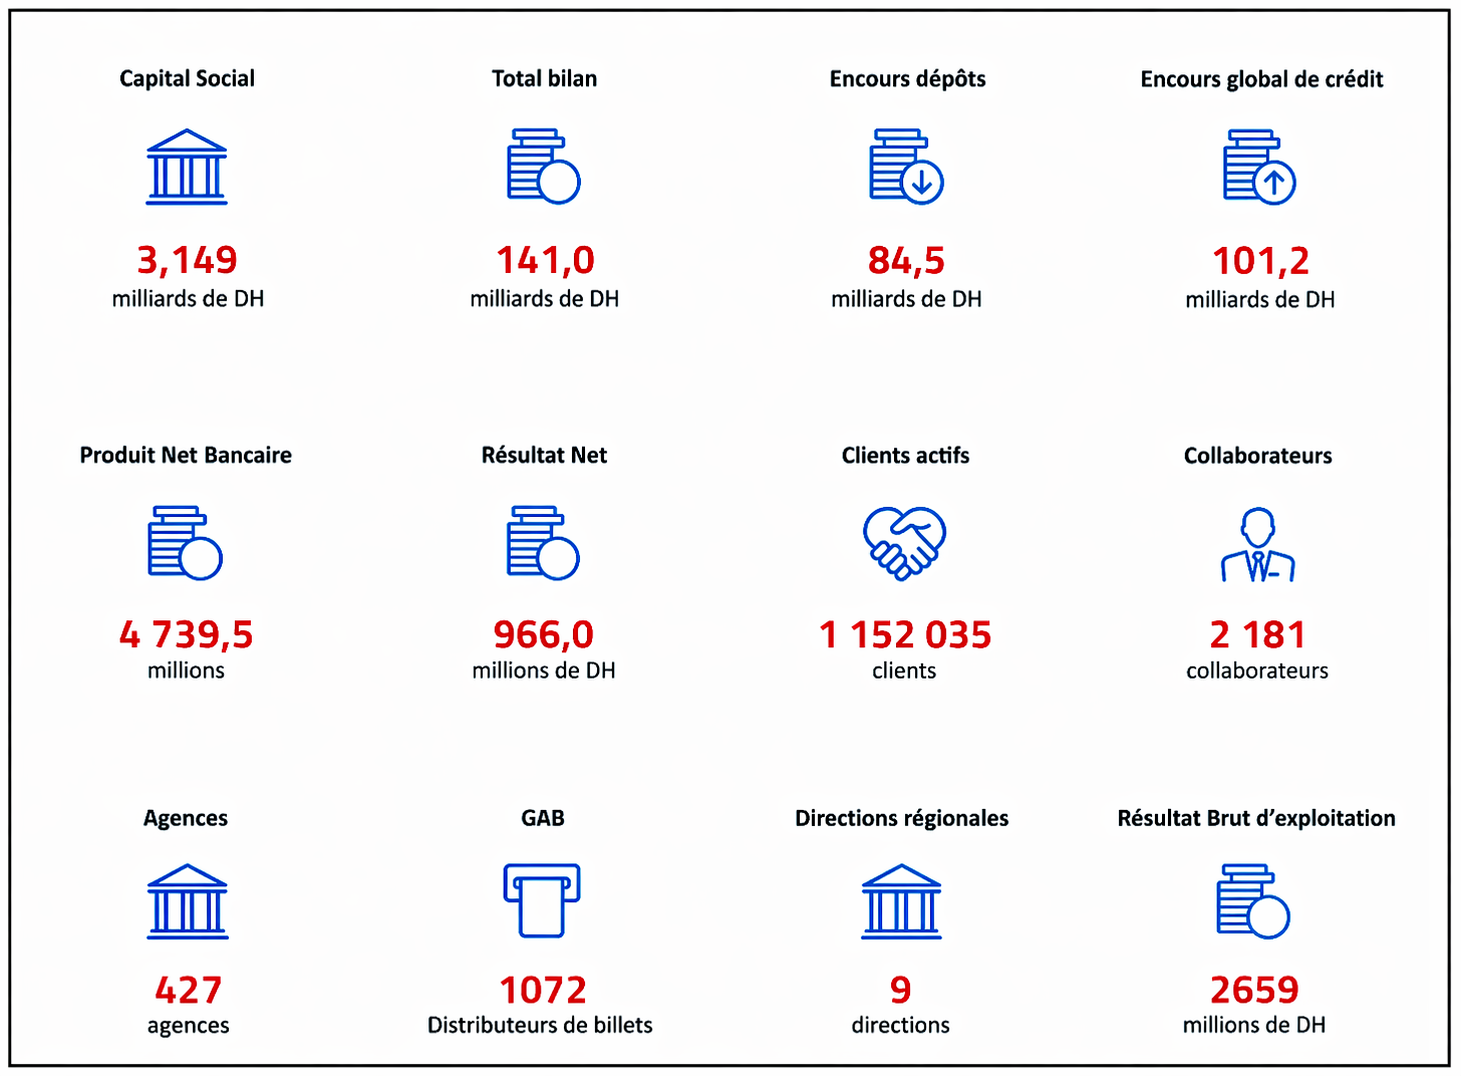
\includegraphics[width=0.8\textwidth]{figures/chiffresCles.png}
    \caption{Chiffres clés de CIH BANK (31/12/2024)}
    \label{fig:chiffres}
\end{figure}

Les chiffres clés de CIH BANK reflètent la situation financière et opérationnelle de l’institution. Avec un capital social de 3,149 milliards de dirhams et un total bilan de 141 milliards de dirhams, la banque dispose d’une base financière significative. L’encours des dépôts s’élève à 84,5 milliards de dirhams, tandis que l’encours global de crédit atteint 101,2 milliards de dirhams. Le produit net bancaire est de 4 739,5 millions de dirhams, avec un résultat net de 966 millions de dirhams et un résultat brut d’exploitation de 2 659 millions de dirhams. La banque compte plus de 1,15 million de clients actifs, 2 181 collaborateurs, 427 agences, 1 072 guichets automatiques et 9 directions régionales. Ces indicateurs fournissent une vue d’ensemble de l’activité, de la structure et des résultats financiers de l’institution.

% =========================
\subsection{Organigramme}

\subsubsection{Structure hiérarchique de CIH BANK}

La structure hiérarchique de CIH BANK s'articule autour d'une direction générale pilotée par le Président Directeur Général, appuyée par des fonctions de support stratégique et de contrôle (Audit, Conformité, Risques, Capital Humain, etc.) ainsi que diverses fonctions rattachées. L'activité commerciale et opérationnelle de la banque est quant à elle répartie en plusieurs pôles métiers majeurs : la Banque des Particuliers et Professionnels, la Banque de l’Entreprise et de l’Immobilier, la Banque de l’Investissement, le Financement \& Recouvrement, et les Services à la Clientèle \& Réseaux.

Parmi ces différentes directions, notre attention se porte plus particulièrement sur l'entité technologique qui encadre notre organisme d'accueil :

\paragraph*{Fonctions technologiques et data}

Au niveau des fonctions technologiques et de gestion de la donnée, le pôle Services Technologiques et Opérations englobe la Sécurité des Systèmes d’Information, la Qualité, ainsi que le Pôle Systèmes d’Information. C'est au sein de la direction Data Management \& Intelligence Artificielle de ce même pôle que se trouve le Data Office, l'entité d'accueil de notre projet de fin d'études.

L'organigramme global de CIH BANK est illustré dans la figure \ref{fig:organigramme} ci-dessous.

\begin{figure}[H]
    \centering
    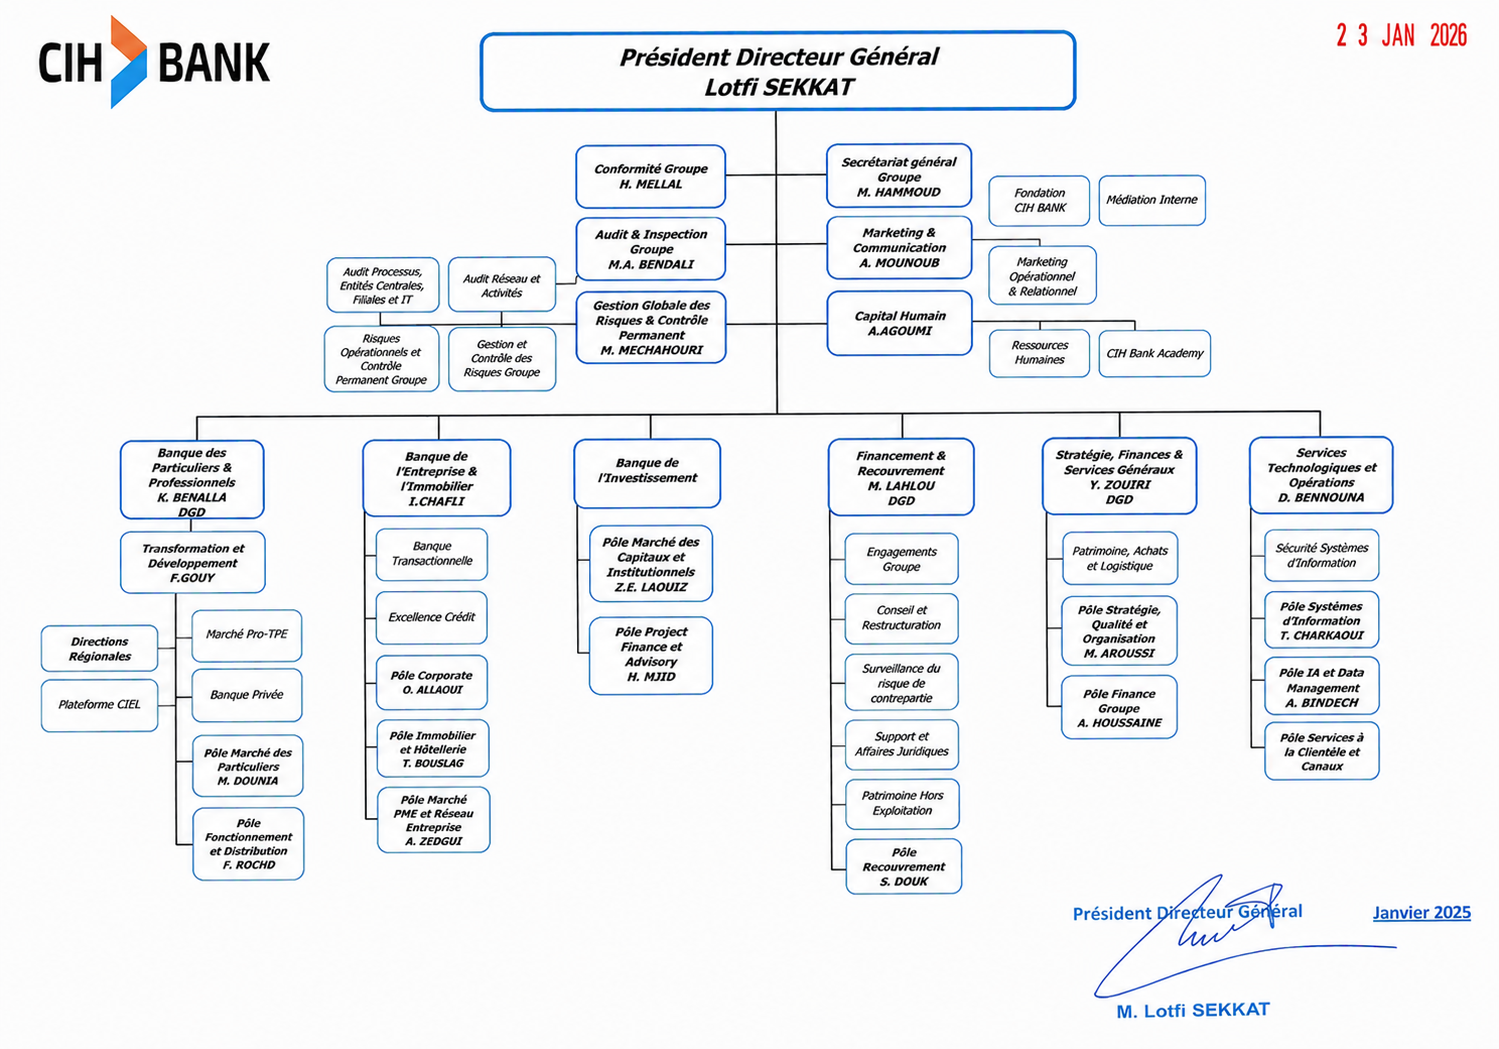
\includegraphics[angle=90, width=\textwidth, height=0.8\textheight, keepaspectratio]{figures/Organigramme.png}
    \caption{Organigramme de CIH BANK}
    \label{fig:organigramme}
\end{figure}

% =========================
\subsection{Data Office}

Dans le cadre de notre stage, nous avons intégré le Data Office de CIH BANK, une entité dédiée à la gestion, au traitement et à la valorisation des données de la banque.

Le Data Office est aujourd’hui rattaché au pôle Services Technologiques et Opérations, plus précisément au sein de la direction Data Management et Intelligence Artificielle. Cette organisation reflète l’importance stratégique accordée à la donnée dans le pilotage des activités de la banque.

Cette entité regroupe plusieurs profils complémentaires intervenant sur l’ensemble du cycle de vie de la donnée. Les \textit{Data Engineers} sont en charge de l’ingestion, du traitement et de la mise à disposition des données. Ils collaborent étroitement avec les \textit{Data Analysts}, responsables de l’analyse et de la production d’indicateurs décisionnels, ainsi qu'avec les \textit{Data Scientists}, spécialisés dans la modélisation avancée et l’analyse prédictive. Enfin, l’équipe \textit{Data Management} assure la gouvernance transversale, la qualité et la structuration des données au sein de la banque.

Les données sont collectées à partir des différents systèmes opérationnels de la banque, puis intégrées et centralisées au sein d’un Data Lake. Elles sont ensuite transformées et mises à disposition pour répondre aux besoins analytiques, réglementaires et métiers.

Dans ce cadre, le Data Office joue un rôle central dans la mise en place des pratiques de gestion de la qualité des données.


% =========================
\section{Étude de l'existant}

\subsection{Description de l'existant}

\subsubsection*{Contexte et enjeux de la qualité des données bancaires}
Dans l'écosystème financier contemporain, la transition vers une économie numérique a redéfini la nature des institutions bancaires. La donnée n'est plus un simple sous-produit de l'activité transactionnelle, mais s'impose comme une infrastructure essentielle sur laquelle reposent l'évaluation des risques, les décisions stratégiques, et une conformité réglementaire extrêmement stricte. Au Maroc, cette conformité s'articule prioritairement autour de la protection des données à caractère personnel, régie par la loi 09-08 de la CNDP (Commission Nationale de contrôle de la protection des Données à caractère Personnel). S'y ajoute le respect du RGPD européen pour la clientèle résidant en Europe, ainsi que d'autres normes internationales liées aux risques (ex: BCBS 239).
Sur le plan économique, le coût de la non-qualité est très élevé. La « règle de dix » (\textit{Rule of Ten}) stipule qu'il coûte dix fois plus cher de corriger une donnée en aval que de la valider directement à la source. Une gouvernance proactive apporte une valeur mesurable : optimisation des fonds propres, efficacité opérationnelle et sécurisation des décisions basées sur l'intelligence artificielle.

\subsubsection*{Le domaine Tiers : Cartographie et données}
Historiquement, la vérification de la qualité des données au sein de CIH BANK était un processus réactif déclenché sur demande, ce qui a motivé la création de l'entité Data Management (DM). Notre projet s'inscrit dans cette volonté d'amélioration continue et cible plus particulièrement le \textbf{Référentiel Tiers}. Ce référentiel regroupe l'ensemble des informations relatives aux personnes physiques et morales en relation avec la banque.

Dans le cadre de l'ingestion des données vers le Data Lake, l'équipe travaille sur plus d'une dizaine de tables du domaine Tiers. À titre d'illustration, les tables principales extraites du système opérant Oracle NOVA (\texttt{CCM}) qui structurent notre périmètre de base sont : \texttt{identity} (pièces d'identité), \texttt{legalentity} (personnes morales), \texttt{person} (statut client), \texttt{professionaldescription} (caractéristiques professionnelles), \texttt{jobs} (catégories socio-professionnelles CSP), ainsi que la table centrale \textbf{\texttt{np\_description}} (Natural Person Description) regroupant les données d'état civil et les informations KYC pour les personnes physiques.

Bien que le pipeline automatisé de qualité de données déployé couvre l'ensemble du domaine Tiers (soit une quinzaine de tables issues de NOVA), \textbf{pour des soucis de clarté et d'illustration, les implémentations techniques et les règles de Data Quality présentées dans la suite de ce rapport se focaliseront particulièrement sur les tables \texttt{np\_description} et \texttt{jobs}}. Ces tables sont éminemment stratégiques : \texttt{np\_description} concentre les données KYC indispensables à l'identification réglementaire du client (nom, prénom, date de naissance, genre, nationalité, etc.), tandis que \texttt{jobs} contient des informations essentielles pour la catégorisation socio-professionnelle (CSP).

\subsubsection*{Architecture et pipeline de données}
L'ensemble des données ingérées au sein de CIH BANK, incluant celles du domaine Tiers, transite par une plateforme robuste centralisée s'appuyant sur une infrastructure Big Data de pointe. Tout l'écosystème analytique repose sur ce système unifié pour le traitement et la valorisation de la donnée.

\begin{figure}[H]
\centering
\includegraphics[width=0.95\textwidth]{figures/Architecture et pipeline de données.png}
\caption{Architecture matérielle Big Data}
\label{fig:architecture_big_data}
\end{figure}

L'architecture matérielle et logicielle de cette plateforme de production s'articule autour d'un \textbf{cluster Cloudera et Dremio} composé de 8 nœuds (3 Masters, 3 Workers, 2 Gateways). Le flux global des données, de la source à l'exploitation, suit un cycle de vie standardisé en plusieurs étapes :

\paragraph{1. Ingestion :} Les données brutes issues des systèmes opérants (Oracle NOVA, PowerCard, etc.) sont ingérées massivement via des scripts \textbf{Apache Sqoop} organisés par domaine métier. Les tables sont stockées au format \textbf{ORC} dans la zone RAW de Hive via HCatalog. L'authentification aux sources s'effectue par \textbf{Kerberos} (\texttt{kinit} avec keytab).

\paragraph{2. Transformation :} Des pipelines PySpark packagés sous forme de fichiers \textbf{Wheel} (\texttt{.whl}), construits via le gestionnaire \textbf{PDM}, effectuent le nettoyage, le renommage des colonnes et l'enrichissement des données brutes pour les charger dans la zone de STAGING. Chaque écriture est tracée par une colonne d'audit \texttt{batch\_time}.

\paragraph{3. Virtualisation et Métadonnées :} Le moteur de données Dremio se connecte aux catalogues (Hive Metastore) pour virtualiser les tables. Il offre une couche sémantique puissante permettant de croiser et d'interroger les données sans les dupliquer.

\paragraph{4. Exposition et Datamarts :} Les données transformées sont consolidées et exposées sous forme de Datamarts (ou vues métiers spécifiques). Ces ensembles de données prêts à l'emploi alimentent les outils de restitution (Tableau) pour répondre aux besoins analytiques des métiers.

\subsection{Critique de l'existant}
Bien que cette infrastructure de production Cloudera soit robuste, l'absence d'un contrôle automatisé de la qualité des données en amont pose plusieurs problèmes majeurs transverses à l'ensemble des tables du domaine Tiers. Pour illustrer l'impact de ces problèmes, nous prenons l'exemple des tables \texttt{np\_description} et \texttt{jobs}, qui contiennent des données KYC et CSP particulièrement sensibles concernant les personnes physiques :

\paragraph{Absence de validation à la source :} Les données transitent vers Dremio sans aucune validation intermédiaire. Des incohérences flagrantes persistent, comme des discordances entre le genre et la civilité du client, ou des dates de naissance remplies par défaut.

\paragraph{Risques de non-conformité réglementaire :} L'absence ou l'invalidité de certains champs critiques, tels que l'identifiant FATCA pour les clients concernés, expose la banque à des risques réglementaires et à d'éventuelles sanctions.

\paragraph{Démarche réactive et manuelle :} Lorsqu'une anomalie est repérée par les métiers en bout de chaîne, la réconciliation implique asynchronement plusieurs équipes pour des corrections curatives chronophages, créant ainsi des processus inefficaces.

\paragraph{Manque de traçabilité et d'historisation :} Aucune métrique n'est historisée dans le temps. Les Data Stewards ne disposent d'aucun outil pour prioriser ou surveiller la santé des données KYC au quotidien.

\subsection{Solution proposée}
Pour pallier ces limites, nous proposons de concevoir et d'implémenter un \textbf{pipeline automatisé de contrôle de la qualité des données} couvrant l'ensemble du périmètre Tiers, intégré directement dans la zone RAW de l'infrastructure Hadoop. La solution technique s'articule autour de trois piliers majeurs :

\paragraph{Automatisation native via Soda Core :} L'intégration de la bibliothèque Soda Core au sein des workflows Airflow existants permet de valider systématiquement les données KYC (exhaustivité, unicité, validité de format, cohérence croisée) dès leur ingestion.

\paragraph{Approche proactive et détection précoce :} En signalant les anomalies dès la zone RAW, nous empêchons l'exploitation de données erronées par les couches analytiques aval, appliquant ainsi le principe de la \textit{Rule of Ten}.

\paragraph{Monitoring centralisé et restitution décisionnelle :} Les résultats des contrôles et les anomalies consolidées sont persistés dans des tables Hive dédiées. Un tableau de bord interactif est ensuite construit pour offrir aux Data Stewards une vue claire de la santé des tables du référentiel, tout en garantissant la stricte anonymisation des données personnelles.

\paragraph{Fondation pour l'Intelligence Artificielle (\textit{Data Readiness for AI}) :} Dans le secteur bancaire, la fiabilité des modèles prédictifs et des algorithmes d'apprentissage automatique (tels que le scoring de risque de crédit, la détection des fraudes ou la segmentation client) est strictement conditionnée par la qualité des données en entrée (\textit{Garbage In, Garbage Out}). En garantissant la complétude et la cohérence des variables fondamentales KYC et CSP dès leur arrivée dans le Data Lake, notre pipeline assure la robustesse des données destinées à alimenter les pipelines de Machine Learning de la banque.

Cette solution permet d'améliorer la gouvernance globale des données du domaine Tiers tout en optimisant le temps de traitement des anomalies.

\section{Choix du modèle de développement}

Pour mener à bien ce projet, nous avons adopté une démarche \textbf{Agile inspirée du framework Scrum, adaptée aux spécificités de l'ingénierie Big Data}. La complexité de l'écosystème distribué et l'étendue du domaine Tiers ont motivé un découpage itératif par livrables fonctionnels (\textit{Minimum Viable Products} et \textit{Proof of Concepts}), permettant d'éprouver et de valider les règles de qualité de manière progressive, table par table.

Sur le plan opérationnel, cette démarche s'est articulée autour d'un rythme adapté : des synchronisations hebdomadaires (\textit{Weekly standups}) avec le \textit{Delivery Manager} pour piloter l'avancement des \textit{backlogs} individuels et lever les verrous techniques, associées à des points de validation réguliers avec le \textit{Data Steward} (agissant en tant que \textit{Product Owner} métier). Cette organisation a assuré une forte réactivité face aux contraintes de l'infrastructure Cloudera tout en maintenant un alignement continu avec les priorités métiers de la banque.

% =========================
\section{Planning prévisionnel}

Afin de mener à bien ce projet au sein du Data Office de CIH BANK, nous avons défini un planning de travail couvrant une période de six mois, du \textbf{9 février au 9 août 2026}. 

Contrairement à un projet classique, l'avancement n'a pas été strictement linéaire. Les deux premiers mois ont été presque exclusivement dédiés à la compréhension fonctionnelle, technique, et à la documentation détaillée de l'architecture existante. Par la suite, les phases de conception, de réalisation des POCs, et de tests se sont superposées de manière itérative, accompagnées de réunions continues avec les métiers.

La figure \ref{fig:gantt} ci-dessous illustre ce déroulement sous forme d'un diagramme de Gantt, mettant en évidence la phase initiale de documentation, le cycle itératif de développement, et l'implication constante des acteurs métiers.

\begin{figure}[H]
    \centering
    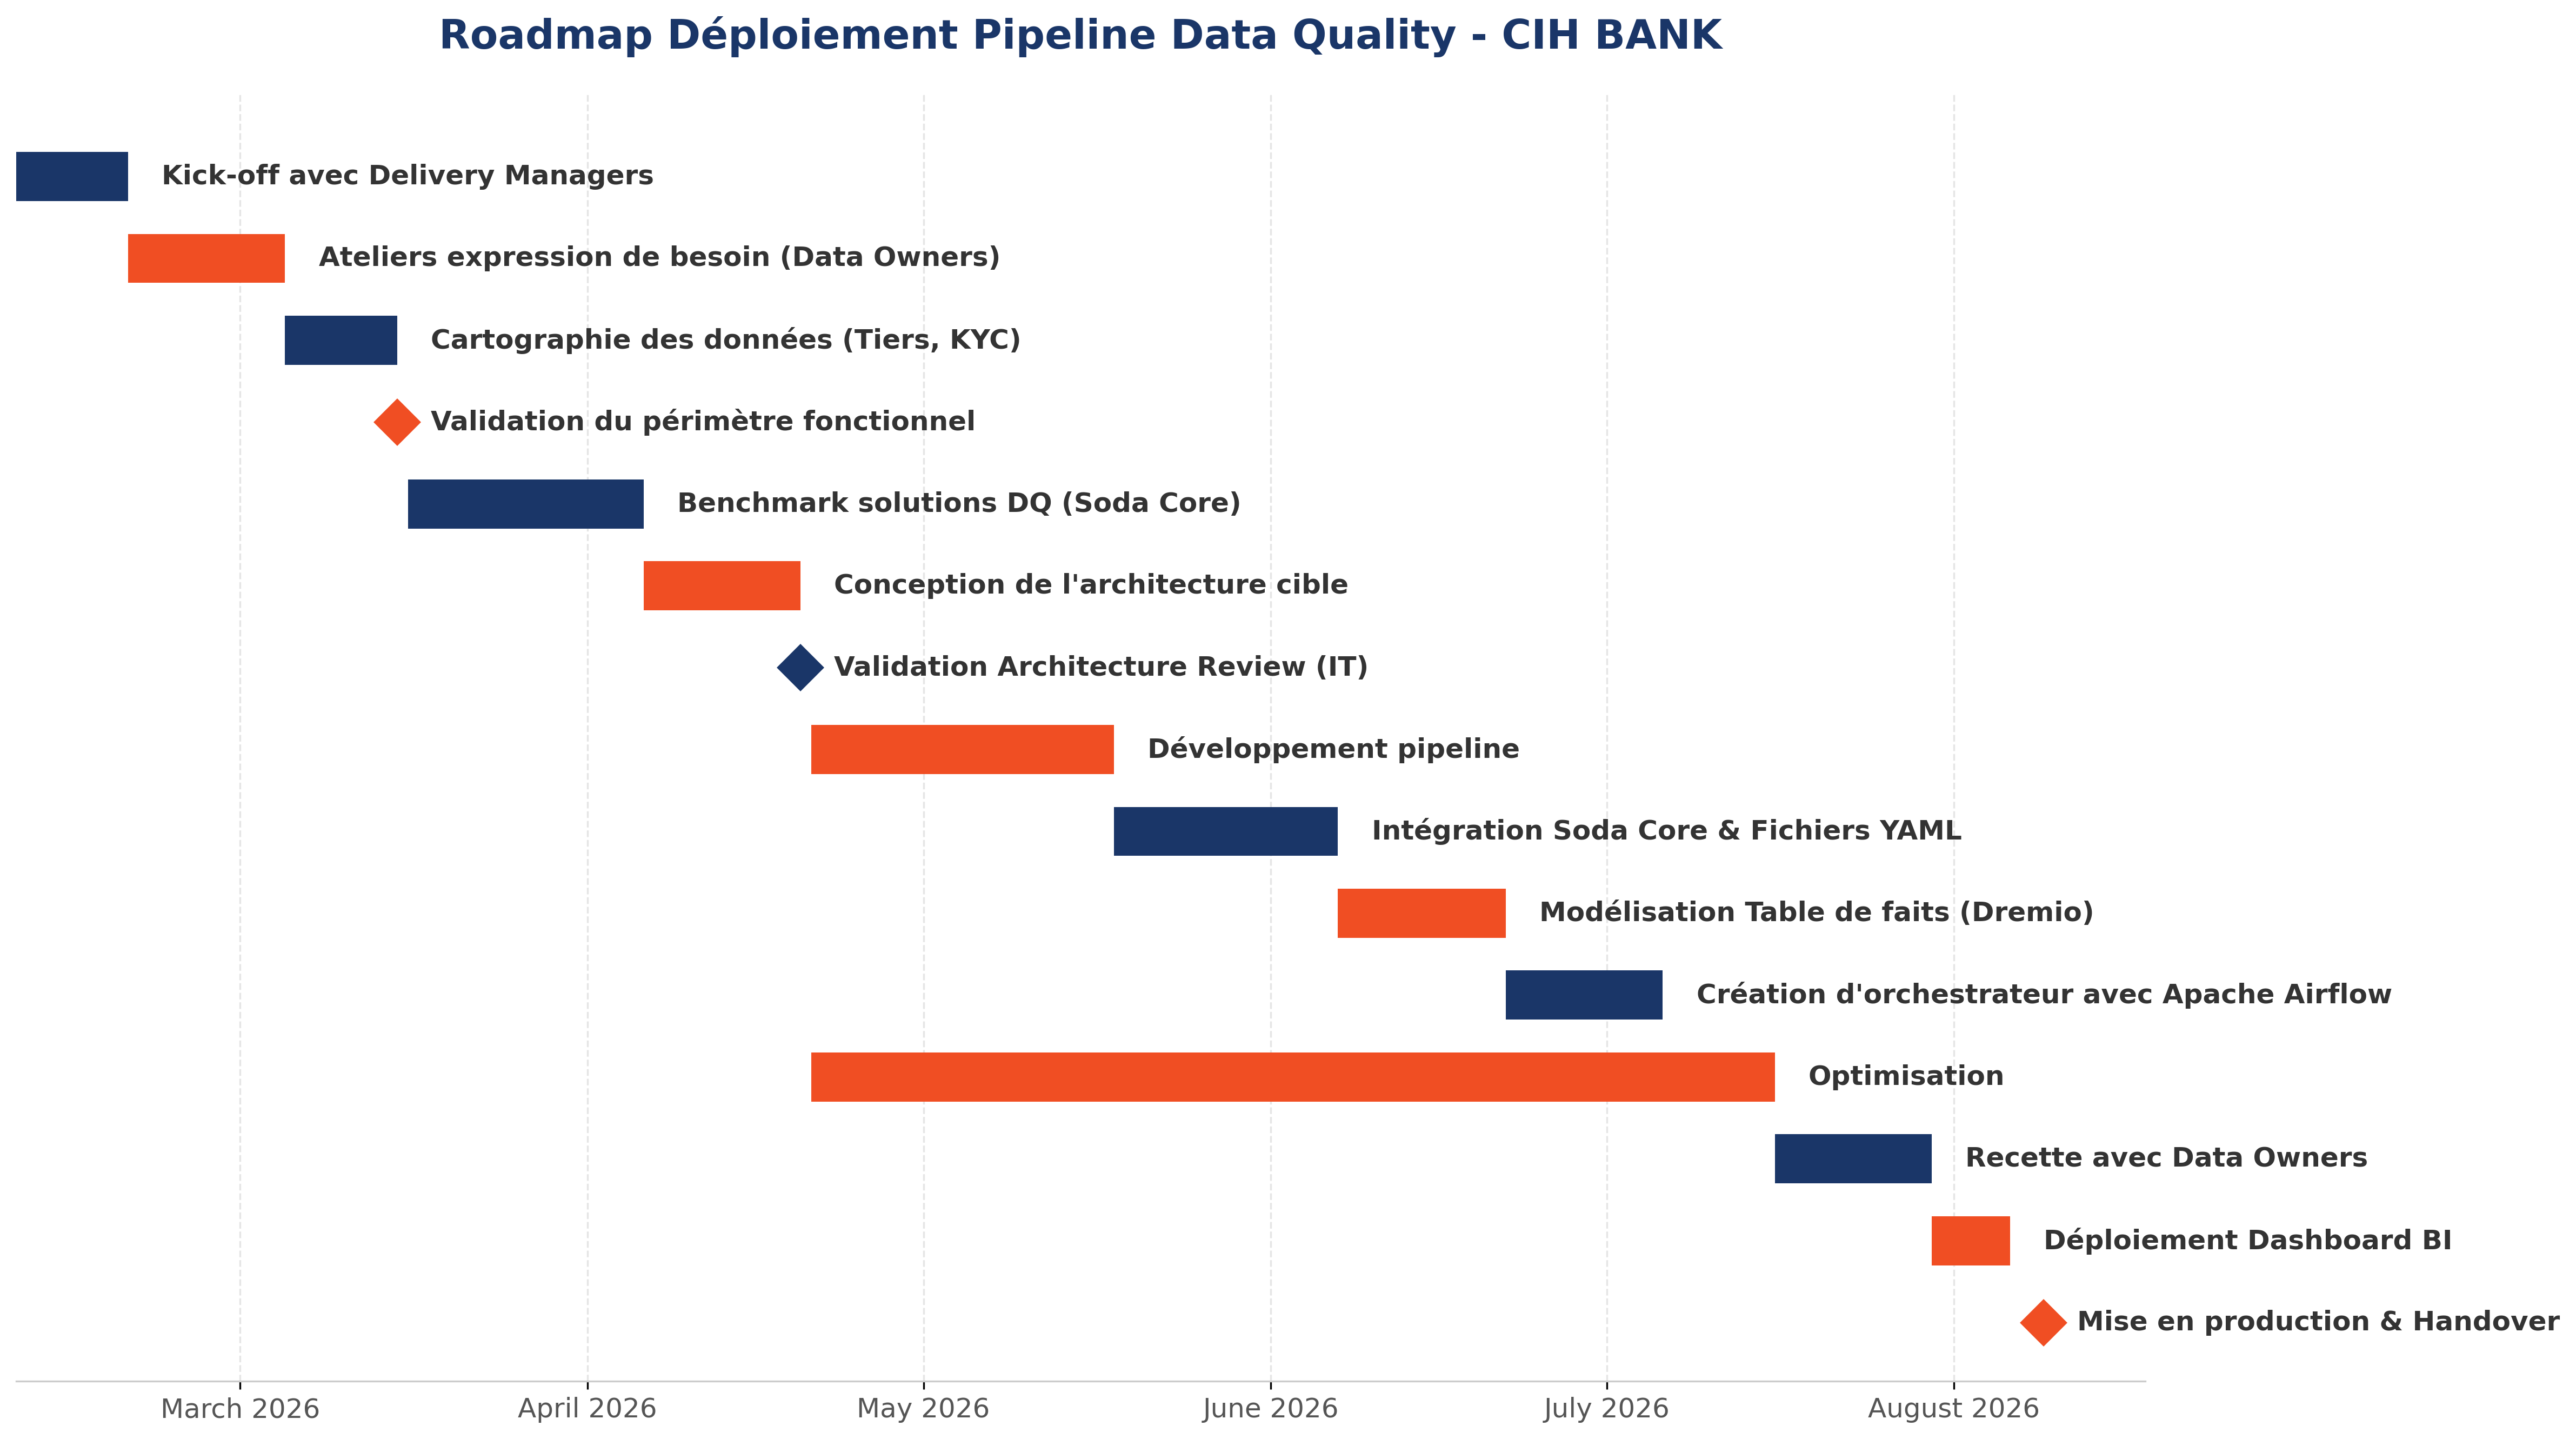
\includegraphics[width=1.0\textwidth]{figures/Gantt_CIH_Bank_Final.png}
    \caption{Planning prévisionnel du projet}
    \label{fig:gantt}
\end{figure}

% =========================
\section*{Conclusion}

Pour conclure, CIH BANK est une institution bancaire marocaine majeure, fortement structurée et engagée dans la valorisation de la donnée à travers son Data Office. L'étude de l'existant a permis de mettre en évidence les processus actuels de gestion des données et leurs limites, ce qui justifie la nécessité d'un pipeline automatisé de contrôle qualité. Ces éléments constituent la base de notre projet et nous permettent d'entamer sereinement la phase de spécification des besoins dans le chapitre suivant.

\chapter{Analyse des Besoins et Spécification}

\section*{Introduction du chapitre}
Après avoir décrit le cadre général du projet et analysé le fonctionnement de la solution existante au sein de CIH BANK, ce chapitre se focalise sur la définition claire et rigoureuse des besoins. Nous y détaillons d'une part les besoins fonctionnels, c'est-à-dire les fonctionnalités attendues du pipeline de Data Quality, et d'autre part les besoins non fonctionnels, liés aux exigences techniques, de performance et de sécurité. Enfin, nous présentons la modélisation fonctionnelle à travers la spécification des cas d'utilisation et de leurs acteurs.

% =========================
\section{Besoins fonctionnels}

Les besoins fonctionnels décrivent les actions que le système doit être capable de réaliser pour répondre aux problématiques de qualité des données identifiées sur le domaine Tiers. Ces problématiques, transverses à l'ensemble des tables du référentiel, seront illustrées par la table \texttt{np\_description} et ses 40 colonnes (\texttt{name}, \texttt{firstname}, \texttt{civility}, \texttt{sex}, \texttt{birthdate}, \texttt{nationalitycountry}, \texttt{fatcaidentificationnumber}, etc.). Les besoins se répartissent en quatre fonctionnalités majeures :

\subsection{Automatisation et planification des contrôles}
\begin{itemize}
    \item \textbf{Sous-besoin 1.1 : Déclenchement automatique} : Le système doit lancer l'évaluation de la qualité des données de manière planifiée, immédiatement après l'exécution complète du batch quotidien d'ingestion des tables sources Oracle NOVA (via un nouveau DAG dédié s'exécutant à 00h00, séparé du DAG d'ingestion \texttt{dailyow22} de 22h00) ,
    \item \textbf{Sous-besoin 1.2 : Orchestration intégrée} : L'exécution du scan de qualité doit être orchestrée au sein d'Apache Airflow, permettant de suivre son statut d'exécution (Succès/Échec) et de consulter les logs en temps réel.
\end{itemize}

\subsection{Configuration déclarative des règles de qualité}
\begin{itemize}
    \item \textbf{Sous-besoin 2.1 : Moteur de règles dynamique} : Le système doit permettre de définir les contrôles de qualité (Missing, Invalid, Freshness, Consistency, Uniqueness) dans des fichiers de règles déclaratifs séparés du code source ,
    \item \textbf{Sous-besoin 2.2 : Graduation des seuils et des alertes} : Pour chaque contrôle, le système doit pouvoir évaluer des seuils paramétrables (ex : taux de valeurs manquantes inférieur à 5\%) et générer un statut de warning ou d'error selon la gravité de l'écart ,
    \item \textbf{Sous-besoin 2.3 : Gestion des métadonnées} : Chaque règle doit être documentée avec des attributs métier (nom de la règle, dimension DQ associée, domaine KYC ou CSP, criticité, etc.).
\end{itemize}

\subsection{Historisation et traçabilité des indicateurs}
\begin{itemize}
    \item \textbf{Sous-besoin 3.1 : Persistance journalière} : À chaque exécution, le système doit sauvegarder les métriques calculées et les résultats de chaque contrôle de qualité dans des tables d'historique de scores (base Hive dédiée \texttt{dq\_results}), indexée par date d'exécution ,
    \item \textbf{Sous-besoin 3.2 : Identification des anomalies (Remédiation)} : Le système doit capturer de manière détaillée la liste des enregistrements clients en anomalie en stockant leur identifiant technique (UUID) et leur radical (numéro client), ainsi que le libellé du contrôle en échec et sa criticité. Ces informations doivent être stockées dans une table d'anomalies pour actions correctives.
\end{itemize}

\subsection{Restitution visuelle et aide à la décision}
\begin{itemize}
    \item \textbf{Sous-besoin 4.1 : Exposition des données} : Les résultats d'historisation de la qualité doivent être exposés de manière transparente sous forme de vues SQL pour les outils décisionnels ,
    \item \textbf{Sous-besoin 4.2 : Suivi de l'évolution temporelle} : Le tableau de bord doit permettre de suivre la tendance d'évolution des scores DQ dans le temps (30 derniers jours) ,
    \item \textbf{Sous-besoin 4.3 : Priorisation des remédiations} : Le tableau de bord doit fournir une liste opérationnelle des clients en anomalie triée par criticité décroissante, exportable par les Data Stewards pour traitement correctif dans le système source NOVA.
\end{itemize}

% =========================
\section{Besoins non fonctionnels}

Les besoins non fonctionnels expriment les exigences qualitatives, opérationnelles et techniques que la solution doit respecter pour être viable et performante dans l'environnement de production de CIH BANK :

\subsection{Performance}
Le Référentiel Tiers de la banque regroupe \textbf{plusieurs millions} de dossiers clients (personnes physiques). Les règles de cohérence inter-colonnes ou de doublons nécessitent des jointures lourdes. Le moteur DQ doit être capable d'interroger et d'évaluer ce volume massif de données en un temps minimal (moins de 15 minutes) sans dégrader les ressources du Data Lake. Cela justifie l'utilisation d'un moteur de calcul distribué (Apache Spark) pour le traitement.

\subsection{Disponibilité}
L'exécution des contrôles de qualité ne doit pas bloquer la disponibilité des données pour les outils de reporting en cas d'anomalie. Si un seuil de qualité est franchi ou si le scan échoue, le pipeline d'exposition (Dremio/Tableau) doit continuer à fonctionner en mode dégradé en signalant l'alerte. De plus, la tâche DQ doit s'exécuter même si certaines tables d'ingestion n'ont été chargées que partiellement.

\subsection{Maintenabilité}
L'ajout de nouvelles règles ou l'intégration de nouvelles colonnes du Référentiel Tiers (par exemple pour de nouveaux critères réglementaires ou pour les personnes morales) doit se faire sans modification du code Python principal de la solution. Les fichiers de configuration YAML et la structure des tables Hive de résultats doivent être conçus de manière générique pour supporter l'extensibilité.

\subsection{Sécurité}
Les détails d'anomalies de qualité des données contiennent des informations clients sensibles (\texttt{name}, \texttt{firstname}, radicaux). Seuls les collaborateurs habilités du Data Office (Data Stewards, Data Project) et les Data Owners des départements concernés doivent être autorisés à accéder aux détails des anomalies. La solution s'appuie sur les mécanismes de sécurité existants de la plateforme :
\begin{itemize}
    \item \textbf{Authentification Kerberos} : L'ensemble des composants du cluster Cloudera (HDFS, Hive, Spark) sont sécurisés par Kerberos, garantissant l'identité de chaque service et utilisateur ,
    \item \textbf{Autorisation Apache Ranger} : Les politiques d'accès aux tables Hive et aux espaces HDFS sont gérées de manière centralisée via Ranger, permettant un contrôle fin par rôle ,
    \item \textbf{Annuaire LDAP / Active Directory} : L'authentification des utilisateurs Dremio et Tableau est déléguée à l'annuaire d'entreprise, assurant une gestion unifiée des identités.
\end{itemize}

% =========================
\section{Modélisation des cas d'utilisation}

\subsection{Acteurs du système}
L'intégration de la solution de Data Quality au sein de CIH BANK repose sur une étroite collaboration entre les experts métier, l'équipe technique et les systèmes d'information. Le tableau \ref{tab:acteurs_dq} présente les cinq acteurs clés du système.

\begin{table}[H]
\centering
\caption{Acteurs du système de Data Quality}
\label{tab:acteurs_dq}
\renewcommand{\arraystretch}{1.4}
\resizebox{\textwidth}{!}{
\begin{tabular}{|l|l|p{9cm}|}
\hline
\rowcolor{gray!20}
\textbf{Acteur} & \textbf{Type} & \textbf{Rôle dans le système DQ} \\
\hline
Équipe Data (DE / Data Steward) & Interne & Organise les ateliers d'alignement, formalise les règles dans les fichiers YAML Soda Core et implémente les flux techniques. \\
\hline
Métiers (Data Owners) & Humain & Experts fonctionnels qui définissent et valident les règles de qualité, consultent le dashboard et remédient aux anomalies. \\
\hline
Équipe SI & Appui & Valide la faisabilité technique des règles vis-à-vis du modèle physique Oracle NOVA. \\
\hline
Airflow (Orchestrateur) & Système & Déclenche automatiquement le scan DQ chaque soir après l'ingestion (nouveau DAG à 00h00). \\
\hline
Oracle NOVA (Système source) & Externe & Récepteur final des corrections de données opérées par les gestionnaires suite aux alertes DQ. \\
\hline
\end{tabular}
}
\end{table}

\subsection{Diagramme global des cas d'utilisation}
Le diagramme ci-dessous synthétise graphiquement les cas d'utilisation du système de Data Quality et les interactions avec les différents acteurs impliqués dans ce cycle de gouvernance.

\begin{figure}[H]
\centering
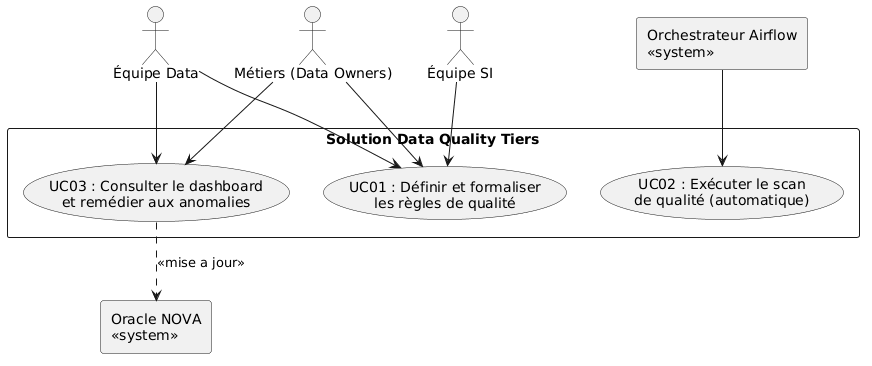
\includegraphics[width=0.95\textwidth]{figures/usecaseGeneral.png}
\caption{Diagramme global des cas d'utilisation de la solution DQ Tiers}
\label{fig:usecase_dq}
\end{figure}

\subsection{Description textuelle des cas d'utilisation principaux}
Nous détaillons ci-dessous le déroulement des trois phases principales constituant le cycle de vie de la qualité des données de notre solution.

\subsubsection{Cas d'utilisation 01 : Définir et formaliser les règles de qualité}

\begin{table}[H]
\centering
\caption{Description du cas d'utilisation 01}
\label{tab:uc01}
\renewcommand{\arraystretch}{1.4}
\begin{tabular}{|l|p{10cm}|}
\hline
\rowcolor{gray!20}
\textbf{Champ} & \textbf{Description} \\
\hline
\textbf{Titre} & Définir et formaliser les règles de qualité \\
\hline
\textbf{Acteurs} & Équipe Data (Steward / DE), Métiers (Data Owners), Équipe SI \\
\hline
\textbf{Préconditions} & Cadrage fonctionnel du domaine Tiers défini \\
\hline
\textbf{Scénario nominal} &
1. L'équipe Data organise des ateliers d'alignement avec les experts Métier et l'équipe SI. \newline
2. Les parties s'accordent sur le catalogue des contrôles (complétude KYC, cohérence CSP) et les seuils de tolérance. \newline
3. L'équipe Data consigne les spécifications dans un document de cadrage. \newline
4. Le Data Engineer implémente les règles dans les fichiers YAML Soda Core. \\
\hline
\textbf{Postconditions} & Les règles de qualité sont formalisées et déployées dans le moteur Soda. \\
\hline
\end{tabular}
\end{table}

\subsubsection{Cas d'utilisation 02 : Exécuter le scan de qualité (automatique)}

\begin{table}[H]
\centering
\caption{Description du cas d'utilisation 02}
\label{tab:uc02}
\renewcommand{\arraystretch}{1.4}
\begin{tabular}{|l|p{10cm}|}
\hline
\rowcolor{gray!20}
\textbf{Champ} & \textbf{Description} \\
\hline
\textbf{Titre} & Exécuter le scan de qualité (automatique) \\
\hline
\textbf{Acteur principal} & Orchestrateur Airflow (Système) \\
\hline
\textbf{Préconditions} & Fin de l'ingestion quotidienne Sqoop des tables NOVA \\
\hline
\textbf{Scénario nominal} &
1. Airflow lance automatiquement la tâche DQ de nuit. \newline
2. Le moteur DQ Soda Core lit les fichiers YAML et exécute les requêtes sur Spark. \newline
3. Les résultats agrégés et les détails des anomalies clients sont historisés dans la base Hive \texttt{dq\_results}. \\
\hline
\textbf{Postconditions} & Les indicateurs et anomalies du jour sont prêts à être exposés. \\
\hline
\end{tabular}
\end{table}

\subsubsection{Cas d'utilisation 03 : Consulter le dashboard et remédier aux anomalies}

\begin{table}[H]
\centering
\caption{Description du cas d'utilisation 03}
\label{tab:uc03}
\renewcommand{\arraystretch}{1.4}
\begin{tabular}{|l|p{10cm}|}
\hline
\rowcolor{gray!20}
\textbf{Champ} & \textbf{Description} \\
\hline
\textbf{Titre} & Consulter le dashboard et remédier aux anomalies \\
\hline
\textbf{Acteurs} & Métiers (Parties prenantes), Data Stewards \\
\hline
\textbf{Préconditions} & Le scan DQ s'est exécuté de manière conforme \\
\hline
\textbf{Scénario nominal} &
1. Le dashboard Tableau se rafraîchit automatiquement chaque matin. \newline
2. Chaque partie prenante consulte le dashboard depuis son poste de travail. \newline
3. Chaque acteur filtre et exporte la liste des anomalies de son périmètre. \newline
4. Les acteurs procèdent à la correction des anomalies dans Oracle NOVA. \\
\hline
\textbf{Postconditions} & Les données corrigées dans NOVA sont ré-ingérées lors du prochain batch et le score DQ s'améliore automatiquement. \\
\hline
\end{tabular}
\end{table}

\section*{Conclusion du chapitre}
Ce chapitre a permis de formaliser les besoins fonctionnels et non fonctionnels, définissant de manière précise les objectifs techniques et opérationnels du pipeline de qualité des données. La modélisation des acteurs et des cas d'utilisation reflète fidèlement le cycle de gouvernance de CIH BANK, où chaque partie prenante collabore d'abord à la définition des contrôles, puis intervient individuellement sur son périmètre pour corriger les anomalies identifiées au quotidien. Fort de ces spécifications, le chapitre suivant présente la conception globale et détaillée de la solution.

\chapter{Conception de la Solution}

\section*{Introduction du chapitre}
Après avoir défini les besoins fonctionnels et non fonctionnels de notre système de contrôle de la qualité des données, ce chapitre présente la conception détaillée de la solution. Conformément aux exigences du Template 2, nous décrivons dans un premier temps la modélisation dynamique à travers des diagrammes de séquences, et d'activités. Dans un second temps, nous présentons la modélisation statique comprenant le diagramme de classes, le modèle relationnel, le dictionnaire de données et le catalogue complet des règles de qualité. Enfin, nous détaillons l'architecture logicielle (diagramme de composants) et matérielle (diagramme de déploiement) de l'application dans son environnement CIH BANK.

% =========================================================================
\section{Modélisation dynamique}

La modélisation dynamique permet de représenter les interactions temporelles entre les différents composants du système et l'évolution des états des données au cours de l'exécution du processus de contrôle.

\subsection{Diagramme de séquences}
Le diagramme de séquences de la figure \ref{fig:sequence_dq} détaille le flux d'exécution séquentiel d'un scan de qualité de données. Il illustre comment la tâche DQ intégrée dans Airflow coordonne le traitement entre la zone HDFS RAW, le moteur Soda Core et la base Hive de résultats, jusqu'à l'exposition finale vers Tableau.

\begin{figure}[H]
    \centering
    \resizebox{\textwidth}{!}{
    \begin{tikzpicture}[node distance=2.6cm, >=stealth, every node/.style={font=\normalsize}]
        % Lifelines
        \node (airflow) [draw=blue!80!black, fill=blue!10, rounded corners, minimum width=2.2cm, minimum height=1cm, drop shadow] {\textbf{Airflow}};
        \node (sqoop) [draw=blue!80!black, fill=blue!10, rounded corners, minimum width=2.2cm, minimum height=1cm, drop shadow, right=of airflow] {\textbf{Sqoop}};
        \node (hdfs) [draw=blue!80!black, fill=blue!10, rounded corners, minimum width=2.2cm, minimum height=1cm, drop shadow, right=of sqoop] {\textbf{Hive / HDFS}};
        \node (soda) [draw=blue!80!black, fill=blue!10, rounded corners, minimum width=2.5cm, minimum height=1cm, drop shadow, right=of hdfs, align=center] {\textbf{Data Quality}\\\textbf{Engine}};
        \node (dremio) [draw=blue!80!black, fill=blue!10, rounded corners, minimum width=2.2cm, minimum height=1cm, drop shadow, right=of soda] {\textbf{Dremio}};
        \node (tableau) [draw=blue!80!black, fill=blue!10, rounded corners, minimum width=2.2cm, minimum height=1cm, drop shadow, right=of dremio] {\textbf{Tableau}};

        % Dotted lines
        \draw [dashed, draw=gray, thick] (airflow) -- +(0,-18.0);
        \draw [dashed, draw=gray, thick] (sqoop) -- +(0,-18.0);
        \draw [dashed, draw=gray, thick] (hdfs) -- +(0,-18.0);
        \draw [dashed, draw=gray, thick] (soda) -- +(0,-18.0);
        \draw [dashed, draw=gray, thick] (dremio) -- +(0,-18.0);
        \draw [dashed, draw=gray, thick] (tableau) -- +(0,-18.0);

        % Execution arrows
        \draw [->, line width=1.2pt] ($(airflow)+(0,-1.8)$) -- node[above, font=\small, text width=2.4cm, align=center] {1. DAG Ingestion (22h00)} ($(sqoop)+(0,-1.8)$);
        
        \draw [->, line width=1.2pt] ($(sqoop)+(0,-3.3)$) -- node[above, font=\small, text width=2.4cm, align=center] {2. Importer données} ($(hdfs)+(0,-3.3)$);
        
        \draw [<-, dashed, line width=1.2pt, color=green!50!black] ($(sqoop)+(0,-4.8)$) -- node[above, font=\small, text width=2.4cm, align=center] {3. OK (Succès)} ($(hdfs)+(0,-4.8)$);
        
        \draw [->, line width=1.2pt] ($(airflow)+(0,-6.3)$) -- node[above, font=\small, text width=4.5cm, align=center] {4. DAG Qualité (00h00)} ($(soda)+(0,-6.3)$);
        
        \draw [->, line width=1.2pt] ($(soda)+(0,-7.8)$) -- node[above, font=\small, text width=2.4cm, align=center] {5. Évaluer règles sur RAW} ($(hdfs)+(0,-7.8)$);
        
        \draw [<-, dashed, line width=1.2pt, color=gray!80!black] ($(soda)+(0,-9.3)$) -- node[above, font=\small, text width=2.4cm, align=center] {6. Données brutes} ($(hdfs)+(0,-9.3)$);
        
        \draw [->, line width=1.2pt] ($(soda)+(0,-10.8)$) -- node[above, font=\small, text width=2.4cm, align=center] {7. Sauvegarder (3 tables)} ($(hdfs)+(0,-10.8)$);
        
        \draw [->, line width=1.2pt] ($(tableau)+(0,-12.3)$) -- node[above, font=\small, text width=2.4cm, align=center] {8. Requêter le Dashboard} ($(dremio)+(0,-12.3)$);
        
        % Arrow from Dremio to HDFS (crosses Soda)
        \draw [->, line width=1.2pt] ($(dremio)+(0,-13.8)$) -- node[above, font=\small, text width=5cm, align=center, pos=0.7] {9. Interroger les 3 tables} ($(hdfs)+(0,-13.8)$);
        
        % Arrow from HDFS to Dremio (crosses Soda)
        \draw [<-, dashed, line width=1.2pt, color=gray!80!black] ($(dremio)+(0,-15.3)$) -- node[above, font=\small, text width=5cm, align=center, pos=0.7] {10. Virtualisation des données} ($(hdfs)+(0,-15.3)$);
        
        \draw [<-, dashed, line width=1.2pt, color=blue!60!black] ($(tableau)+(0,-16.8)$) -- node[above, font=\small, text width=2.4cm, align=center] {11. Vues consolidées} ($(dremio)+(0,-16.8)$);
        
    \end{tikzpicture}
    }
    \caption{Diagramme de séquences du pipeline de contrôle et restitution DQ}
    \label{fig:sequence_dq}
\end{figure}



\subsection{Diagramme d'activités}
Le diagramme d'activités présenté dans la figure \ref{fig:activity_dq} décrit le processus de bout en bout de traitement de la qualité, depuis le chargement initial des données en zone RAW HDFS jusqu'à la remédiation effective dans l'application source Oracle NOVA.

\begin{figure}[H]
    \centering
    \resizebox{0.9\textwidth}{!}{
    \begin{tikzpicture}[
        >=stealth, 
        every node/.style={font=\normalsize}, 
        block/.style={draw=blue!80!black, rectangle, rounded corners, fill=blue!5, minimum width=4cm, minimum height=1.2cm, align=center, drop shadow, thick}, 
        decision/.style={draw=orange!80!black, diamond, aspect=2.5, fill=yellow!10, minimum width=3cm, minimum height=1.5cm, align=center, drop shadow, thick}
    ]
        % Nodes
        \node (start) [draw, circle, fill=black, inner sep=3pt] at (0,0) {};
        \node (ingest) [block] at (0,-1.5) {\textbf{Ingestion HDFS RAW} \\ (Données Tiers via Sqoop)};
        \node (scan) [block] at (0,-3.3) {\textbf{Exécution Soda Core} \\ (Évaluation des règles DQ)};
        \node (dec) [decision] at (0,-5.5) {\textbf{Anomalies} \\ \textbf{détectées ?}};
        \node (score_ok) [block, fill=green!10, draw=green!60!black] at (6,-5.5) {\textbf{Validation} \\ Score = 100\%};
        \node (score_fail) [block, fill=red!10, draw=red!60!black] at (0,-7.8) {\textbf{Échec (Alerte)} \\ Historisation de l'anomalie};
        \node (remed) [block, fill=purple!10, draw=purple!60!black] at (0,-9.8) {\textbf{Correction Manuelle} \\ (Action par le Data Steward \\ dans Oracle NOVA)};
        \node (end) [draw, circle, double=black, fill=black, inner sep=3pt] at (6,-7.8) {};

        % Arrows
        \draw [->, thick] (start) -- (ingest);
        \draw [->, thick] (ingest) -- (scan);
        \draw [->, thick] (scan) -- (dec);
        \draw [->, thick, color=green!60!black] (dec) -- node[above, font=\small, text=green!60!black, font=\bfseries] {Non (0 erreur)} (score_ok);
        \draw [->, thick, color=red!60!black] (dec) -- node[right, font=\small, text=red!60!black, font=\bfseries] {Oui (> 0)} (score_fail);
        \draw [->, thick] (score_fail) -- (remed);
        \draw [->, thick] (score_ok) -- (end);
        
        % Loop back
        \draw [->, thick, dashed] (remed) .. controls (-4.5,-9.8) and (-4.5,-1.5) .. node[left, font=\small, align=center, xshift=-0.2cm] {Nouveau passage\\(J+1)} (ingest);
    \end{tikzpicture}
    }
    \caption{Diagramme d'activités du workflow de remédiation DQ}
    \label{fig:activity_dq}
\end{figure}

% =========================================================================
\section{Modélisation statique}

La modélisation statique définit la structure fixe du système, ses composants de données, le schéma relationnel de stockage de l'historique de qualité, ainsi que le dictionnaire des métadonnées associées.


\subsection{Modélisation de la table de faits}
Étant donné que la solution s'articule autour de la manipulation de données (Data Management) et non d'un développement orienté objet, nous remplaçons le diagramme de classes traditionnel par une modélisation explicite de la table de faits. 

La figure \ref{fig:fact_dq} illustre la structure des données générée par notre moteur de qualité. Le moteur Soda Core produit un ensemble de trois tables physiques liées par l'identifiant d'exécution (\texttt{run\_id} et \texttt{query\_id}). Ces trois tables sont ensuite unifiées au sein de Dremio pour exposer une grande table de faits consolidée (21 colonnes) servant de source unique de vérité pour le reporting BI.

\begin{figure}[H]
    \centering
    \resizebox{\textwidth}{!}{
    \begin{tikzpicture}[
        every node/.style={font=\small}, 
        tablebox/.style={draw, rectangle split, rectangle split parts=2, fill=blue!5, rounded corners, align=left, drop shadow, text width=5.8cm},
        factbox/.style={draw, rectangle split, rectangle split parts=2, fill=green!10, rounded corners, align=left, drop shadow, text width=6.5cm, line width=1.2pt, draw=green!50!black}
    ]
        
        % Central Fact Table
        \node (fact) [factbox] {
            \centering \textbf{fact\_tiers\_dq\_consolidated} \\ (Vue Dremio - 21 colonnes)
            \nodepart{second}
            \textbf{Clés de jointure :}\\
            - Run\_ID \hfill \textit{String}\\
            - Query\_ID \hfill \textit{String}\\
            \midrule
            \textbf{Indicateurs métier (History) :}\\
            - Date de run \hfill \textit{Date}\\
            - Table \hfill \textit{String}\\
            - Colonne \hfill \textit{String}\\
            - Domaine \hfill \textit{String}\\
            - Règle \hfill \textit{String}\\
            - Score Qualité (\%) \hfill \textit{Double}\\
            - Statut (PASS/WARN/FAIL) \hfill \textit{String}\\
            - Criticité \hfill \textit{String}\\
            - Volume Total \hfill \textit{Long}\\
            - Lignes Conformes \hfill \textit{Long}\\
            \midrule
            \textbf{Configuration (Config) :}\\
            - Requête SQL exécutée \hfill \textit{String}\\
            - Chemin Virtuel Complet \hfill \textit{String}\\
            \midrule
            \textbf{Statuts techniques (Log) :}\\
            - Check Execution Status \hfill \textit{String}\\
            - Check Error Message \hfill \textit{String}\\
            - Run Execution Status \hfill \textit{String}\\
            - Run Error Message \hfill \textit{String}\\
            - Date Mise à jour \hfill \textit{Timestamp}
        };

        % Top Table (History)
        \node (colhist) [tablebox, above=of fact, yshift=1.5cm] {
            \centering \textbf{consolidated\_all\_column\_history} \\ (Table physique Hive)
            \nodepart{second}
            + run\_id \textbf{[PK]} \hfill \textit{String}\\
            + query\_id \textbf{[PK]} \hfill \textit{String}\\
            + colonne\_controlee \hfill \textit{String}\\
            + chemin\_source \hfill \textit{String}\\
            + table\_dataset \hfill \textit{String}\\
            + domaine\_metier \hfill \textit{String}\\
            + type\_regle\_dq \hfill \textit{String}\\
            + volume\_total \hfill \textit{Long}\\
            + lignes\_conformes \hfill \textit{Long}\\
            + score\_qualite\_pct \hfill \textit{Double}\\
            + statut \hfill \textit{String}\\
            + date\_execution \hfill \textit{Timestamp}\\
            + criticite \hfill \textit{String}
        };

        % Bottom Left Table (Checks Config)
        \node (checks) [tablebox, below left=of fact, xshift=-1cm, yshift=-1.5cm] {
            \centering \textbf{consolidated\_all\_checks\_config} \\ (Table physique Hive)
            \nodepart{second}
            + run\_id \textbf{[PK]} \hfill \textit{String}\\
            + query\_id \textbf{[PK]} \hfill \textit{String}\\
            + run\_date \hfill \textit{Date}\\
            + table \hfill \textit{String}\\
            + domain \hfill \textit{String}\\
            + rule \hfill \textit{String}\\
            + virt\_col \hfill \textit{String}\\
            + virt\_full\_path \hfill \textit{String}\\
            + raw\_col \hfill \textit{String}\\
            + sql \hfill \textit{String}\\
            + updated\_at \hfill \textit{Timestamp}\\
            + criticite \hfill \textit{String}
        };

        % Bottom Right Table (Execution Log)
        \node (exec) [tablebox, below right=of fact, xshift=1cm, yshift=-1.5cm] {
            \centering \textbf{consolidated\_execution\_log} \\ (Table physique Hive)
            \nodepart{second}
            + run\_id \textbf{[PK]} \hfill \textit{String}\\
            + query\_id \textbf{[PK]} \hfill \textit{String}\\
            + run\_date \hfill \textit{Date}\\
            + table \hfill \textit{String}\\
            + domain \hfill \textit{String}\\
            + rule \hfill \textit{String}\\
            + virt\_col \hfill \textit{String}\\
            + virt\_full\_path \hfill \textit{String}\\
            + raw\_col \hfill \textit{String}\\
            + check\_execution\_status \hfill \textit{String}\\
            + check\_error\_message \hfill \textit{String}\\
            + check\_timestamp \hfill \textit{Timestamp} \\
            + run\_execution\_status \hfill \textit{String}\\
            + run\_error\_message \hfill \textit{String}\\
            + updated\_at \hfill \textit{Timestamp}
        };

        % Arrows pointing to the central fact table
        \draw[->, line width=1.5pt, draw=gray!80, >=stealth] (colhist.south) -- node[right, font=\footnotesize\bfseries, text=gray!80] {Virtualisation Dremio} (fact.north);
        \draw[->, line width=1.5pt, draw=gray!80, >=stealth] (checks.north east) -- (fact.south west);
        \draw[->, line width=1.5pt, draw=gray!80, >=stealth] (exec.north west) -- (fact.south east);
        
    \end{tikzpicture}
    }
    \caption{Modélisation de la grande table de faits \texttt{fact\_tiers\_dq\_consolidated} et ses 3 tables sources}
    \label{fig:fact_dq}
\end{figure}

\subsection{Modèle relationnel}
Pour persister les résultats d'évaluation de la qualité des données, nous concevons un schéma physique relationnel indépendant au sein de la base de données Hive, basé sur trois tables distinctes :
\begin{itemize}
    \item \textbf{consolidated\_all\_column\_history} : Table principale d'historisation des indicateurs et scores de qualité par exécution, table et colonne. Elle inclut la criticité métier du contrôle.
    \item \textbf{consolidated\_all\_checks\_config} : Table de configuration stockant la requête SQL générée par le moteur pour chaque règle évaluée, ainsi que sa criticité.
    \item \textbf{consolidated\_execution\_log} : Table de journalisation technique traçant le succès ou l'échec d'exécution du contrôle.
\end{itemize}



\subsection{Dictionnaire de données}
Les attributs clés de ces trois tables sont consolidés via Dremio pour fournir un ensemble de 21 colonnes à Tableau. Voici les colonnes principales exploitées :

\begin{table}[H]
\centering
\caption{Dictionnaire simplifié des tables de faits de Qualité des Données}
\label{tab:dict_results_fact}
\renewcommand{\arraystretch}{1.3}
\resizebox{\textwidth}{!}{
\begin{tabular}{|l|l|p{8cm}|}
\hline
\rowcolor{gray!20}
\textbf{Colonne} & \textbf{Table source} & \textbf{Description / Rôle} \\
\hline
\texttt{run\_id} & Toutes & Identifiant unique de l'exécution du processus DQ. \\
\hline
\texttt{query\_id} & Toutes & Identifiant de la requête ou de la règle évaluée. \\
\hline
\texttt{type\_regle\_dq} & \texttt{column\_history} & Dimension DQ (ex: Completude, Conformite, Coherence...). \\
\hline
\texttt{criticite} & \texttt{column\_history} / \texttt{checks\_config} & Niveau de criticité du contrôle (CRITIQUE, HAUTE, MOYENNE). \\
\hline
\texttt{domaine\_metier} & \texttt{column\_history} & Domaine métier visé (PTP-TIE-POR). \\
\hline
\texttt{score\_qualite\_pct} & \texttt{column\_history} & Taux de conformité en pourcentage. \\
\hline
\texttt{statut} & \texttt{column\_history} & État d'évaluation métier de la règle (PASS, WARN, FAIL). \\
\hline
\texttt{sql} & \texttt{checks\_config} & Requête SQL exécutée par le moteur SparkSQL. \\
\hline
\texttt{check\_execution\_status} & \texttt{execution\_log} & Statut d'exécution technique du job (SUCCESS/ERROR). \\
\hline
\end{tabular}
}
\end{table}

\subsection{Catalogue des règles de qualité}
Les contrôles de qualité s'appliquent sur l'ensemble des données du domaine Tiers (informations KYC et données socioprofessionnelles CSP). Afin d'offrir une structuration claire et directement exploitable, le catalogue des règles de gestion est organisé par \textbf{dimension de Data Quality} : Complétude, Conformité, Cohérence, Unicité et Actualité / Pipeline.

L'établissement de ce catalogue découle d'une analyse exploratoire approfondie menée sur un échantillon réel de 5 000 dossiers de personnes physiques issus de la table \texttt{ccm\_npdescription}. Cette analyse a révélé des anomalies typiques et récurrentes de saisie au sein du système opérant Oracle NOVA, ce qui a directement guidé le choix et le paramétrage de nos dimensions de contrôle :
\begin{itemize}
    \item \textbf{Le phénomène des dates de naissance génériques} : Une forte concentration de dates de naissance au premier janvier (\texttt{01/01/YYYY}) a été identifiée (par exemple \texttt{1947-01-01}, \texttt{1961-01-01}), traduisant une saisie par défaut dans NOVA lorsque seule l'année de naissance est connue. Cela justifie notre règle de validité sur \texttt{birthdate} avec un seuil de tolérance de 15\% ,
    \item \textbf{Le codage numérique des villes} : Le champ \texttt{birthcity} contient des codes numériques (comme \texttt{787}) au lieu de libellés textuels, nécessitant un contrôle de validité par rapport au référentiel des villes pour assurer la cohérence et la résolubilité des codes ,
    \item \textbf{La cohérence conditionnelle FATCA} : L'identifiant FATCA (\texttt{fatcaidentificationnumber}) est majoritairement nul, ce qui est cohérent pour les citoyens marocains (\texttt{nationalitycountry = MA}), mais doit être obligatoirement renseigné pour les clients ayant la nationalité ou une double nationalité américaine.
\end{itemize}

\subsubsection{Dimension Complétude}
La dimension de complétude mesure le taux de renseignement des attributs obligatoires pour assurer l'exploitabilité opérationnelle des dossiers clients.

\begin{longtable}{|p{0.20\textwidth}|p{0.30\textwidth}|p{0.14\textwidth}|p{0.30\textwidth}|}
\caption{Dimension Complétude — Données Tiers (KYC \& CSP)} \label{tab:completude_tiers} \\
\hline
\rowcolor{gray!20}
\textbf{Colonne(s)} & \textbf{Description Règle / Seuil} & \textbf{Criticité} & \textbf{Action corrective} \\
\hline
\endfirsthead
\hline
\rowcolor{gray!20}
\textbf{Colonne(s)} & \textbf{Description Règle / Seuil} & \textbf{Criticité} & \textbf{Action corrective} \\
\hline
\endhead
\texttt{name} & 0 valeur nulle tolérée & CRITIQUE & Audit dossiers - Blocage saisie agence \\
\hline
\texttt{firstname} & 0 valeur nulle tolérée & CRITIQUE & Audit dossiers - Blocage saisie agence \\
\hline
\texttt{birthdate} & 0 valeur nulle tolérée & CRITIQUE & Saisie obligatoire avec justificatif officiel \\
\hline
\texttt{nationality\_}\allowbreak\texttt{country} & 0 valeur nulle tolérée & HAUTE & Renseigner le code pays de nationalité \\
\hline
\texttt{professional\_}\allowbreak\texttt{sector} & Taux de valeurs nulles < 5\% & HAUTE & Renseigner le secteur d'activité de l'employeur \\
\hline
\texttt{occupation} & Taux de valeurs nulles < 5\% & HAUTE & Préciser la profession exacte du client \\
\hline
\texttt{socioprofessional\_}\allowbreak\texttt{category} & Taux de valeurs nulles < 5\% & HAUTE & Renseigner la catégorie socioprofessionnelle (CSP) \\
\hline
\texttt{professional\_}\allowbreak\texttt{situation} & Taux de valeurs nulles < 5\% & HAUTE & Renseigner le statut de la situation professionnelle \\
\hline
\texttt{employer} & Taux de valeurs nulles < 10\% & HAUTE & Renseigner le nom de l'entreprise employeuse \\
\hline
\texttt{politically\_}\allowbreak\texttt{exposed} & 0 valeur nulle tolérée (PEP obligatoire) & CRITIQUE & Renseigner la déclaration d'exposition politique \\
\hline
\end{longtable}

\subsubsection{Dimension Conformité}
La dimension de validité évalue le respect des formats de saisie, des plages de valeurs autorisées et la conformité par rapport aux référentiels métier (BAM, ISO).

\begin{longtable}{|p{0.20\textwidth}|p{0.30\textwidth}|p{0.14\textwidth}|p{0.30\textwidth}|}
\caption{Dimension Conformité — Données Tiers (KYC \& CSP)} \label{tab:validite_tiers} \\
\hline
\rowcolor{gray!20}
\textbf{Colonne(s)} & \textbf{Description Règle / Seuil} & \textbf{Criticité} & \textbf{Action corrective} \\
\hline
\endfirsthead
\hline
\rowcolor{gray!20}
\textbf{Colonne(s)} & \textbf{Description Règle / Seuil} & \textbf{Criticité} & \textbf{Action corrective} \\
\hline
\endhead
\texttt{name}, \texttt{firstname} & Longueur $\ge$ 2, aucun chiffre ou caractère spécial & HAUTE & Nettoyage et normalisation dans NOVA \\
\hline
\texttt{birthdate} & Taux de dates génériques au 01/01 < 15\% & HAUTE & Recherche de la date réelle sur pièce d'identité \\
\hline
\texttt{civility} & Valeurs restreintes à (M., MME, MLLE) & HAUTE & Restauration de la valeur selon pièces fournies \\
\hline
\texttt{sex} & Valeurs restreintes à (M, F) & HAUTE & Restauration de la valeur selon pièces fournies \\
\hline
\texttt{birth\_city} & Doit exister dans le référentiel des villes BAM & MOYENNE & Mapping et correction via la table de transcodage \\
\hline
\texttt{professional\_}\allowbreak\texttt{sector} & Code numérique valide dans le référentiel sectoriel & MOYENNE & Transcodage vers les codes officiels BAM \\
\hline
\texttt{professional\_}\allowbreak\texttt{situation} & Valeurs restreintes à (SAL, FON, TRI, AUT, EMP, NDE) & HAUTE & Remplacer par un code référentiel valide \\
\hline
\texttt{employer} & Détection des valeurs parasites ('AUTRE', 'LUI MEME') & HAUTE & Normaliser : mapper 'LUI MEME' vers auto-entrepreneur \\
\hline
\end{longtable}

\subsubsection{Dimension Cohérence}
La dimension de cohérence vérifie l'absence de contradiction logique entre plusieurs attributs interdépendants.

\begin{longtable}{|p{0.20\textwidth}|p{0.30\textwidth}|p{0.14\textwidth}|p{0.30\textwidth}|}
\caption{Dimension Cohérence — Données Tiers (KYC \& CSP)} \label{tab:coherence_tiers} \\
\hline
\rowcolor{gray!20}
\textbf{Colonne(s)} & \textbf{Description Règle / Seuil} & \textbf{Criticité} & \textbf{Action corrective} \\
\hline
\endfirsthead
\hline
\rowcolor{gray!20}
\textbf{Colonne(s)} & \textbf{Description Règle / Seuil} & \textbf{Criticité} & \textbf{Action corrective} \\
\hline
\endhead
\texttt{sex} + \texttt{civility} & Genre M $\neq$ MME/MLLE ; Genre F $\neq$ M. & CRITIQUE & Résolution manuelle des incohérences de saisie \\
\hline
\texttt{fatca\_}\allowbreak\texttt{identification\_}\allowbreak\texttt{number} & Si nationalité ou double nationalité = US, 0 valeur nulle & CRITIQUE & Déclaration réglementaire FATCA immédiate \\
\hline
\texttt{employer} + \texttt{professional\_}\allowbreak\texttt{situation} & Si situation = NDE (sans emploi) ou TRI (retraité), employeur doit être NULL & HAUTE & Annuler le nom d'employeur incohérent dans NOVA \\
\hline
\end{longtable}

\subsubsection{Dimension Unicité}
La dimension d'unicité contrôle l'absence de doublons d'enregistrements et garantit l'unicité des identifiants principaux du référentiel.

\begin{longtable}{|p{0.20\textwidth}|p{0.30\textwidth}|p{0.14\textwidth}|p{0.30\textwidth}|}
\caption{Dimension Unicité — Données Tiers (KYC \& CSP)} \label{tab:unicite_tiers} \\
\hline
\rowcolor{gray!20}
\textbf{Colonne(s)} & \textbf{Description Règle / Seuil} & \textbf{Criticité} & \textbf{Action corrective} \\
\hline
\endfirsthead
\hline
\rowcolor{gray!20}
\textbf{Colonne(s)} & \textbf{Description Règle / Seuil} & \textbf{Criticité} & \textbf{Action corrective} \\
\hline
\endhead
\texttt{oid} / \texttt{radical} & Unicité stricte du numéro de radical client (0 doublon) & CRITIQUE & Fusion des doublons clients dans le référentiel \\
\hline
\texttt{ordnum} & Un seul enregistrement actif principal (\texttt{main=1}) par tiers & HAUTE & Éliminer les contrats de travail multiples actifs \\
\hline
\end{longtable}

\subsubsection{Dimension Actualité et Pipeline}
La dimension de fraîcheur s'assure du bon cadencement de l'ingestion quotidienne et de l'intégrité de la chaîne technique.

\begin{longtable}{|p{0.20\textwidth}|p{0.30\textwidth}|p{0.14\textwidth}|p{0.30\textwidth}|}
\caption{Dimension Actualité et Pipeline — Flux Batch} \label{tab:regles_fraicheur} \\
\hline
\rowcolor{gray!20}
\textbf{Colonne(s)} & \textbf{Description Règle / Seuil} & \textbf{Criticité} & \textbf{Action corrective} \\
\hline
\endfirsthead
\hline
\rowcolor{gray!20}
\textbf{Colonne(s)} & \textbf{Description Règle / Seuil} & \textbf{Criticité} & \textbf{Action corrective} \\
\hline
\endhead
\texttt{batch\_}\allowbreak\texttt{datetime} & Retard d'ingestion HDFS RAW < 26h & HAUTE & Alerte infrastructure Big Data et relance Sqoop \\
\hline
\texttt{row\_count} & Écart de volumétrie entre Oracle NOVA et Hive RAW < 0.1\% & CRITIQUE & Rejouer le DAG d'ingestion Sqoop \\
\hline
\texttt{code\_segment} & Cohérence entre segment client et code\_marche & HAUTE & Recalculer le segment par défaut \\
\hline
\end{longtable}

% =========================================================================
\section{Architecture de l'application}

L'architecture présente la structure logique de la solution DQ et son déploiement physique sur l'infrastructure de production de CIH BANK.

\subsection{Architecture logicielle (diagramme de composants)}
L'architecture logicielle de notre solution s'articule autour de modules découplés. Le diagramme de la figure \ref{fig:components_dq} illustre les interactions entre les modules d'ingestion, de stockage, de contrôle, de virtualisation et de restitution de la solution.

\begin{figure}[H]
    \centering
    \resizebox{\textwidth}{!}{
    \begin{tikzpicture}[>=stealth, every node/.style={font=\small}, box/.style={draw=blue!80!black, rectangle, fill=blue!5, rounded corners, minimum width=2.8cm, minimum height=1cm, align=center, drop shadow}]
        % Orchestrators
        \node (dag_ing) [box, fill=orange!10, draw=orange!60!black] {DAG Ingestion \\ \scriptsize(22h00)};
        \node (dag_dq) [box, fill=orange!10, draw=orange!60!black, below=of dag_ing, yshift=-1.0cm] {Nouveau DAG DQ \\ \scriptsize(00h00)};
        
        % Components
        \node (ingest) [box, right=of dag_ing, xshift=1.5cm] {Module d'Ingestion \\ \scriptsize(Apache Sqoop)};
        \node (lake) [box, right=of ingest, xshift=0.5cm] {Zone de Stockage RAW \\ \scriptsize(Hive / HDFS)};
        
        \node (soda) [box, right=of dag_dq, xshift=1.5cm] {Moteur DQ \\ \scriptsize(Soda Core / Python)};
        \node (res) [box, right=of soda, xshift=0.5cm] {Résultats DQ \\ \scriptsize(Hive / HDFS)};
        
        \node (dremio) [box, below=of res, yshift=-0.5cm] {Couche de Virtualisation \\ \scriptsize(Dremio)};
        \node (tableau) [box, left=of dremio, xshift=-1.5cm] {Dashboard \\ \scriptsize(Tableau)};

        % Connectors
        \draw [->, line width=1pt, dashed, orange!80!black] (dag_ing) -- node[above, font=\scriptsize] {Déclenche} (ingest);
        \draw [->, line width=1pt, dashed, orange!80!black] (dag_dq) -- node[above, font=\scriptsize] {Déclenche} (soda);
        
        \draw [->, line width=1pt, blue!70!black] (ingest) -- node[above, font=\scriptsize] {Écrit} (lake);
        \draw [->, line width=1pt, blue!70!black] (soda) -- node[right, font=\scriptsize, align=center, pos=0.3] {Scan} (lake);
        \draw [->, line width=1pt, blue!70!black] (soda) -- node[above, font=\scriptsize] {Enregistre} (res);
        \draw [->, line width=1pt, blue!70!black] (dremio) -- node[right, font=\scriptsize] {Virtualise} (res);
        \draw [->, line width=1pt, blue!70!black] (tableau) -- node[above, font=\scriptsize] {Requête} (dremio);
    \end{tikzpicture}
    }
    \caption{Diagramme de composants logiciels de la solution DQ}
    \label{fig:components_dq}
\end{figure}

Les composants clés de cette architecture logicielle sont détaillés ci-dessous :

\subsubsection{Conception du moteur DQ — Soda Core}
Le moteur de contrôle s'appuie sur le framework open source Soda Core, spécifiquement la bibliothèque Python \texttt{soda-core} et son connecteur Spark \texttt{soda-core-spark}. Afin d'assurer une exécution optimale dans notre écosystème Big Data, la conception logicielle repose sur les principes d'intégration suivants :
\begin{itemize}
    \item \textbf{Encapsulation PySpark et Vues Temporaires} : Le script d'exécution principal (\texttt{dq\_tiers\_checks.py}) initialise une session Spark locale. Pour chaque table de la zone RAW à contrôler (ex: \texttt{ccm\_npdescription} et \texttt{ccm\_job}), la session Spark charge la table sous forme de DataFrame PySpark, puis l'enregistre en tant que vue temporaire en mémoire via la méthode \texttt{createOrReplaceTempView()}. Cela permet à Soda Core d'exécuter l'analyse de qualité directement sur ces vues mémoire sans poser de verrous ou d'accès concurrents sur les tables Hive physiques ,
    \item \textbf{Définition déclarative des règles (SodaCL)} : Les contrôles de qualité sont externalisés dans des fichiers de règles YAML exploitant le langage déclaratif SodaCL. Les fichiers sont séparés logiquement par domaine : \texttt{checks\_kyc.yml} pour le KYC, \texttt{checks\_csp.yml} pour les données socio-professionnelles, et \texttt{checks\_pipeline.yml} pour les indicateurs techniques et la fraîcheur ,
    \item \textbf{Extraction programmatique et typage des métadonnées} : Après l'exécution du scan, le script Python exploite les structures d'API de Soda Core (l'objet \texttt{Scan}) pour parcourir la liste des vérifications évaluées. Pour chaque règle, le script extrait dynamiquement le résultat (succès/échec), la valeur de la métrique, le seuil, la dimension (Completeness, Validity, Consistency), le domaine et la criticité (définis en tant qu'attributs personnalisés dans le YAML). Un score de conformité sur 100 est attribué pour chaque règle ,
    \item \textbf{Persistance partitionnée dans trois tables Hive} : Après l'exécution du scan, le script consolide les résultats et écrit dans trois tables physiques Hive distinctes : \texttt{consolidated\_all\_column\_history} pour les résultats, \texttt{consolidated\_all\_checks\_config} pour la configuration et les requêtes SQL générées, et \texttt{consolidated\_execution\_log} pour la journalisation technique.
\end{itemize}

\subsubsection{Conception de l'orchestration Airflow}
La planification, le déclenchement et le monitoring des scans de qualité sont gérés par un \textbf{nouveau DAG Airflow indépendant}, spécifiquement dédié au contrôle DQ. Afin de découpler totalement l'ingestion de la vérification de la qualité, ce nouveau DAG est planifié pour s'exécuter quotidiennement à \textbf{00h00}. Cela laisse une marge de sécurité de deux heures après le déclenchement du DAG d'ingestion Sqoop principal (\texttt{dailyow22}, prévu à 22h00). L'architecture d'exécution repose sur un déclenchement direct du moteur d'évaluation Python Soda Core depuis Airflow. Cette séparation modulaire assure qu'une défaillance dans le DAG d'ingestion ne bloque pas ou ne corrompt pas la supervision de la qualité.


\subsubsection{Conception du dashboard Tableau}
La restitution visuelle est structurée dans un dashboard Tableau interactif connecté en direct au dataset virtuel unique de Dremio. L'intelligence analytique (calcul des scores quotidiens moyens, taux de conformité globaux, regroupements par dimension de qualité ou par date) est configurée à l'aide de feuilles de calcul (sheets) et de filtres dynamiques directement dans Tableau Desktop, tirant parti de la table de faits unique. Le dashboard est structuré en quatre onglets fonctionnels :
\begin{enumerate}
    \item \textbf{Vue Exécutive} : Présente les KPIs de conformité globaux et les alertes critiques pour les Data Owners et la Direction ,
    \item \textbf{Détail KYC} : Permet une analyse fine par colonne et par dimension de qualité sur le domaine KYC ,
    \item \textbf{Détail CSP} : Restitue les scores de conformité socioprofessionnelle et l'évaluation des valeurs parasites ,
    \item \textbf{Anomalies \& Remédiation} : Présente une synthèse des règles et colonnes présentant des taux d'anomalies élevés (filtrée sur \texttt{state != 'pass'}), aidant les Data Stewards à cibler les actions correctives collectives dans NOVA.
\end{enumerate}
Pour des raisons évidentes de sécurité et de conformité réglementaire (notamment les directives de Bank Al-Maghrib et la protection des données personnelles), toutes les données nominatives et les radicaux clients affichés dans les onglets opérationnels font l'objet d'un masquage ou d'un floutage systématique, garantissant la stricte confidentialité des informations sensibles.

\begin{figure}[H]
    \centering
    \begin{tikzpicture}
        \draw[draw=gray, dashed, fill=gray!5, thick, rounded corners] (0,0) rectangle (12,4);
        \node at (6,2) [align=center, text=gray] {\textbf{Capture d'écran à insérer} \\ \small Connexion de Tableau Desktop avec la source Dremio};
    \end{tikzpicture}
    \caption{Connexion en direct de Tableau Desktop avec le dataset virtuel Dremio}
    \label{fig:screenshot_tableau_conn}
\end{figure}

\subsection{Architecture matérielle (diagramme de déploiement)}
Le diagramme de déploiement de la figure \ref{fig:deploy_dq} modélise l'architecture système et l'infrastructure distribuée de production sur laquelle est déployée notre solution au sein de CIH BANK.

\begin{figure}[H]
    \centering
    \begin{tikzpicture}[
        node distance=0.8cm and 1.2cm, 
        >=stealth, 
        every node/.style={font=\scriptsize},
        box/.style={
            draw=blue!60!black, 
            fill=blue!5, 
            rounded corners=4pt, 
            minimum width=3.0cm, 
            minimum height=1.1cm, 
            align=center, 
            line width=0.8pt
        }
    ]
        % Nodes
        \node (client) [box] {\textbf{Poste Data Steward} \\ \tiny Tableau Desktop / Web};
        \node (edge) [box, right=of client] {\textbf{Edge Node (Gateway)} \\ \tiny Airflow / Dremio Coordinator \\ \tiny Hive Metastore};
        \node (master) [box, above right=of edge, yshift=-0.3cm] {\textbf{Master Nodes (x3)} \\ \tiny HDFS NameNode \\ \tiny YARN ResourceManager};
        \node (worker) [box, below right=of edge, yshift=0.3cm] {\textbf{Worker Nodes (x3)} \\ \tiny HDFS DataNodes \\ \tiny YARN NodeManagers};

        % Connectors with style
        \draw [<->, thick, blue!80!black] (client) -- (edge);
        \draw [<->, thick, blue!80!black] (edge) -- (master.west);
        \draw [<->, thick, blue!80!black] (edge) -- (worker.west);
        \draw [<->, thick, dashed, gray] (master) -- (worker);
    \end{tikzpicture}
    \caption{Architecture matérielle et déploiement dans le cluster Big Data}
    \label{fig:deploy_dq}
\end{figure}

Le cluster Big Data Cloudera CDP 7.1.7 de production de CIH BANK est structuré autour de 8 nœuds distribués, configurés de la manière suivante :
\begin{itemize}
    \item \textbf{1 Nœud Edge (Gateway) principal} : Ce serveur sert de point d'entrée pour l'administration et l'orchestration des jobs. Il héberge les workers d'Apache Airflow, le coordinateur Dremio, ainsi que le service Hive Metastore. C'est sur ce nœud qu'est installé l'environnement virtuel Python contenant les packages \texttt{soda-core} et \texttt{soda-core-spark} ,
    \item \textbf{3 Nœuds Masters} : Ils assurent la haute disponibilité du stockage (HDFS NameNodes configurés en Actif/Standby et JournalNodes) et la coordination de l'ordonnancement distributed. Ils hébergent également le YARN ResourceManager pour la répartition des ressources du cluster ,
    \item \textbf{3 Nœuds Workers} : Ces serveurs gèrent le stockage local physique sous HDFS (DataNodes) et disposent des YARN NodeManagers pour allouer des conteneurs de calcul lors de l'exécution distribuée de nos requêtes PySpark et Dremio Executors.
\end{itemize}

\subsubsection{Orchestration technique et protocole de sécurité Kerberos}
Afin de sécuriser les accès aux données confidentielles du domaine Tiers de CIH BANK, l'exécution de la solution de qualité s'intègre au protocole de sécurité global du cluster :
\begin{itemize}
    \item \textbf{Authentification Kerberos} : Le cluster Cloudera étant sécurisé par Kerberos, l'autorisation d'accès aux répertoires HDFS RAW nécessite un ticket d'authentification valide. Avant de lancer le traitement, la tâche Airflow utilise le fichier keytab chiffré (\texttt{tiers\_dq.keytab}) associé au compte de service du domaine Tiers (\texttt{tiers\_dq\_service}) pour générer et renouveler automatiquement le ticket Kerberos via la commande système \texttt{kinit} ,
    \item \textbf{Soumission du job Spark sur YARN} : Le script Python principal est exécuté en mode \texttt{spark-submit} avec le gestionnaire de ressources YARN configuré en mode \texttt{client} depuis le nœud Edge. Le driver Spark s'exécute ainsi localement sur le Gateway Node (dans le process Airflow), tandis que YARN ResourceManager alloue de manière distribuée des exécuteurs Spark au sein des nœuds Workers. Ces exécuteurs lisent et traitent en parallèle les partitions des fichiers HDFS de la zone RAW Hive.
\end{itemize}

% =========================================================================
\subsection{Technologies de l'écosystème utilisées}

Pour s'insérer au mieux au sein du système d'information décisionnel et Big Data de CIH BANK, notre solution exploite les briques technologiques de l'écosystème du Data Lake. Ces technologies sont résumées ci-dessous.

\vspace{0.4cm}

\noindent
\begin{minipage}[c]{0.12\textwidth}
    \centering
    
\includegraphics[width=\textwidth, height=1.0cm, keepaspectratio]{figures/logos/logo_oracle.png}
\end{minipage}
\hspace{0.03\textwidth}
\begin{minipage}[c]{0.83\textwidth}
    \textbf{Oracle NOVA} --- Système opérant source\\
    {\small Base de données relationnelle hébergeant le Core Banking de la banque. Il s'agit du point d'entrée unique des données des clients physiques et moraux (Référentiel Tiers) et de la cible finale de correction.}
\end{minipage}

\vspace{0.4cm}\noindent\rule{\textwidth}{0.2pt}\vspace{0.3cm}

\noindent
\begin{minipage}[c]{0.12\textwidth}
    \centering
    
\includegraphics[width=\textwidth, height=1.0cm, keepaspectratio]{figures/logos/logo_sqoop.png}
\end{minipage}
\hspace{0.03\textwidth}
\begin{minipage}[c]{0.83\textwidth}
    \textbf{Apache Sqoop} --- Ingestion batch Oracle vers HDFS\\
    {\small Technologie d'ingestion permettant le transfert en masse des tables NOVA vers l'infrastructure Hadoop de manière planifiée.}
\end{minipage}

\vspace{0.4cm}\noindent\rule{\textwidth}{0.2pt}\vspace{0.3cm}

\noindent
\begin{minipage}[c]{0.12\textwidth}
    \centering
    
\includegraphics[width=\textwidth, height=1.0cm, keepaspectratio]{figures/logos/logo_airflow.png}
\end{minipage}
\hspace{0.03\textwidth}
\begin{minipage}[c]{0.83\textwidth}
    \textbf{Apache Airflow} --- Orchestrateur de tâches\\
    {\small Outil d'orchestration permettant de planifier, ordonnancer et superviser l'exécution du flux d'ingestion et des scans de qualité de manière centralisée.}
\end{minipage}

\vspace{0.4cm}\noindent\rule{\textwidth}{0.2pt}\vspace{0.3cm}

\noindent
\begin{minipage}[c]{0.12\textwidth}
    \centering
    
\includegraphics[width=\textwidth, height=1.0cm, keepaspectratio]{figures/logos/logo_hadoop.png}
\end{minipage}
\hspace{0.03\textwidth}
\begin{minipage}[c]{0.83\textwidth}
    \textbf{HDFS / Apache Hive} --- Plateforme de stockage et de requêtage\\
    {\small HDFS assure le stockage persistant distribué tandis que Hive structure ces répertoires sous forme de tables SQL relationnelles cibles pour nos contrôles.}
\end{minipage}

\vspace{0.4cm}\noindent\rule{\textwidth}{0.2pt}\vspace{0.3cm}

\noindent
\begin{minipage}[c]{0.12\textwidth}
    \centering
    
\includegraphics[width=\textwidth, height=1.0cm, keepaspectratio]{figures/logos/logo_soda.png}
\end{minipage}
\hspace{0.03\textwidth}
\begin{minipage}[c]{0.83\textwidth}
    \textbf{Soda Core} --- Moteur de contrôle de la qualité (Python)\\
    {\small Framework de validation de données déclaratif basé sur des fichiers YAML de règles de gestion et exécuté programmatiquement sur les tables Hive RAW.}
\end{minipage}

\vspace{0.4cm}\noindent\rule{\textwidth}{0.2pt}\vspace{0.3cm}

\noindent
\begin{minipage}[c]{0.12\textwidth}
    \centering
    
\includegraphics[width=\textwidth, height=1.0cm, keepaspectratio]{figures/logos/logo_dremio.png}
\end{minipage}
\hspace{0.03\textwidth}
\begin{minipage}[c]{0.83\textwidth}
    \textbf{Dremio} --- Moteur de virtualisation et d'exposition\\
    {\small Permet de virtualiser les tables de résultats Hive et d'exposer des vues SQL rapides et sécurisées, éliminant le besoin de dupliquer ou de transférer physiquement les volumes de données.}
\end{minipage}

\vspace{0.4cm}\noindent\rule{\textwidth}{0.2pt}\vspace{0.3cm}

\noindent
\begin{minipage}[c]{0.12\textwidth}
    \centering
    
\includegraphics[width=\textwidth, height=1.0cm, keepaspectratio]{figures/logos/logo_tableau.png}
\end{minipage}
\hspace{0.03\textwidth}
\begin{minipage}[c]{0.83\textwidth}
    \textbf{Tableau} --- Outil d'analyse décisionnelle et Visualisation\\
    {\small Solution BI standard de CIH BANK, connectée en direct à Dremio pour fournir un reporting réactif sur la qualité des tiers à l'intention des Data Owners.}
\end{minipage}

\vspace{0.4cm}

% =========================================================================
\section*{Conclusion du chapitre}
Ce chapitre a décrit la conception complète de la solution de contrôle de la qualité du domaine Tiers. Nous avons structuré la dynamique d'exécution de nos scans et le cycle de vie des anomalies identifiées. La modélisation statique a fourni le diagramme de classes de nos indicateurs, le schéma relationnel et le catalogue complet des règles KYC et CSP de la solution. Enfin, l'architecture logicielle (composants) et matérielle (déploiement) a été détaillée au sein de l'environnement de production. Le chapitre suivant présente l'implémentation physique et les résultats opérationnels obtenus.

\chapter{Réalisation de la Solution}

\section*{Introduction}
Ce chapitre présente la réalisation concrète du pipeline de Data Quality sur le Référentiel Tiers de CIH Bank. Tous les contrôles Soda Core s'effectuent exclusivement sur la \textbf{zone RAW} du Data Lake (base Hive \texttt{raw\_nova\_referentieltiers}), qui constitue la copie exacte et non transformée des tables \texttt{CCM\_*} du système opérant Oracle NOVA (\textbf{\uline{le périmètre complet englobe environ 15 tables Tiers ; dans ce chapitre, les tables \texttt{ccm\_npdescription} et \texttt{ccm\_job} serviront d'exemples illustratifs}}). Nous détaillerons successivement l'environnement technique de développement, l'implémentation du script Soda Core, la création des tables Hive de persistance, l'intégration dans un DAG Airflow indépendant, la mise en place des vues Dremio et la réalisation du dashboard Tableau.

% =========================
\section{Environnement technique de développement}

\subsection{Environnement Hadoop et cluster}

Le développement et les tests ont été réalisés dans l'environnement Hadoop de CIH Bank. L'accès aux tables Hive et aux fichiers HDFS est effectué via les interfaces disponibles dans l'environnement Data Office, en utilisant les comptes de service existants du domaine Tiers.

Les versions exactes des composants utilisés dans l'environnement de production sont les suivantes :

\begin{table}[H]
\centering
\begin{tabular}{|l|l|}
\hline
\rowcolor{gray!20}
\textbf{Composant} & \textbf{Version} \\
\hline
Cloudera Data Platform (CDP) & Private Cloud Base 7.1.7 \\
\hline
Apache Hadoop (HDFS / YARN) & 3.1.1 \\
\hline
Apache Hive & 3.1.3 \\
\hline
Apache Spark & 3.2.0 \\
\hline
Apache Airflow & 2.5.1 \\
\hline
Dremio & Enterprise Edition 2026 \\
\hline
Python & 3.9.13 \\
\hline
Soda Core & soda-core-spark 3.0.45 \\
\hline
Tableau Desktop & Professional Edition 2024.1.2 \\
\hline
\end{tabular}
\caption{Versions des composants de l'environnement technique}
\label{tab:versions_composants}
\end{table}

\subsection{Installation hors-ligne de Soda Core}

La politique stricte de sécurité des systèmes d'information (PSSI) de CIH BANK impose une isolation réseau (air-gap) des serveurs du cluster Big Data, interdisant par conséquent tout accès direct à Internet. L'exécution standard de la commande \texttt{pip install} pour rapatrier les dépendances depuis le registre public PyPI est donc impossible.

L'installation de Soda Core et de son connecteur Spark a donc été réalisée via une procédure d'installation hors-ligne (Offline Wheel Installation) :
\begin{enumerate}
    \item \textbf{Téléchargement des archives (Wheels)} : Sur un poste de travail disposant d'un accès à Internet, les archives des paquets \texttt{soda-core} et \texttt{soda-core-spark} ainsi que l'ensemble de leurs sous-dépendances ont été téléchargées au format \texttt{.whl} dans un dossier dédié.
    \item \textbf{Transfert sécurisé} : Le dossier d'archives a été contrôlé puis transféré de manière sécurisée (SFTP/SCP) vers le nœud Edge (Gateway) du cluster.
    \item \textbf{Installation locale} : Sur le nœud Edge, les paquets ont été déployés dans l'environnement virtuel Python (venv) alloué à l'orchestrateur Airflow à l'aide de la commande \texttt{pip}, en forçant la recherche locale :
\end{enumerate}

\begin{lstlisting}[language=bash]
source /opt/airflow/venv_dq/bin/activate
pip install --no-index --find-links=./soda_wheels soda-core-spark
\end{lstlisting}

Cette méthode garantit la reproductibilité de l'environnement de contrôle tout en respectant scrupuleusement les contraintes de sécurité bancaires.

% =========================
\section{Implémentation du moteur DQ — Soda Core}

\subsection{Structure des fichiers du projet DQ}

Le projet DQ est organisé selon l'arborescence suivante :

\begin{lstlisting}
dq_tiers/
|-- dq_tiers_checks.py          # Script principal Python
|-- checks/
|   |-- checks_tiers.yml        # Regles DQ fonctionnelles Tiers
|   |-- checks_csp.yml          # Regles DQ colonnes CSP
|   +-- checks_pipeline.yml     # Regles fraicheur & pipeline
+-- utils/
    +-- hive_writer.py          # Module d'ecriture resultats dans Hive
\end{lstlisting}

\subsection{Fichier de configuration YAML — Règles Métier (\texttt{checks\_tiers.yml})}

\begin{lstlisting}[language=YAML]
# checks_tiers.yml
# Regles Data Quality - Domaine Tiers
# Source : raw_nova_referentieltiers.ccm_npdescription (zone RAW)
# Zone RAW = copie exacte d'Oracle NOVA, aucune transformation appliquee

checks for ccm_npdescription:

  # --- Completude ---
  - missing_count(name) = 0:
      name: "KYC-01 | Completude | Nom"
      fail: error
      attributes:
        criticite: CRITIQUE
        domaine: KYC
        dimension: completeness

  - missing_count(first_name) = 0:
      name: "KYC-02 | Completude | Prenom"
      fail: error
      attributes:
        criticite: CRITIQUE
        domaine: KYC
        dimension: completeness

  - missing_count(birthdate) = 0:
      name: "KYC-03 | Completude | Date de naissance"
      fail: error
      attributes:
        criticite: CRITIQUE
        domaine: KYC
        dimension: completeness

  - missing_count(nationality_country) = 0:
      name: "KYC-04 | Completude | Nationalite"
      fail: warn
      attributes:
        criticite: HAUTE
        domaine: KYC
        dimension: completeness

  # --- Validite ---
  - invalid_count(civility) = 0:
      valid values: ["M.", "MME", "MLLE"]
      name: "KYC-05 | Validite | Civilite hors referentiel"
      fail: warn
      attributes:
        criticite: HAUTE
        domaine: KYC
        dimension: validity

  - invalid_count(gender) = 0:
      valid values: ["M", "F"]
      name: "KYC-06 | Validite | Genre hors referentiel"
      fail: warn
      attributes:
        criticite: HAUTE
        domaine: KYC
        dimension: validity

  # --- Fraicheur ---
  - freshness(batch_datetime_eaac4) < 26h:
      name: "KYC-07 | Fraicheur | Retard batch"
      fail: error
      attributes:
        criticite: HAUTE
        domaine: PIPELINE
        dimension: freshness
\end{lstlisting}



\subsection{Script Python principal (\texttt{dq\_tiers\_checks.py})}

\begin{lstlisting}[language=Python]
# dq_tiers_checks.py
# Pipeline de Data Quality - Referentiel Tiers PP Clients - Zone RAW
# CIH Bank - Data Office
# Auteur : Saad BENDAHOU
# Declenchement : Nouveau DAG Indépendant (00h00)

import argparse
import datetime
from datetime import date
from pyspark.sql import SparkSession
from soda.scan import Scan

def run_dq_checks(run_date: str):
    """
    Execute les controles DQ Soda Core sur les tables Hive
    du domaine Tiers et persiste les resultats.
    """
    # --- 1. Initialisation de la SparkSession ---
    spark = SparkSession.builder \
        .appName("DQ_Tiers_Checks") \
        .enableHiveSupport() \
        .getOrCreate()

    # --- 2. Initialisation du scan Soda Core ---
    scan = Scan()
    scan.set_data_source_name("hive_raw")
    scan.add_spark_session(spark, "hive_raw")

    # --- 3. Chargement des fichiers de regles YAML ---
    scan.add_sodacl_yaml_file("checks/checks_kyc.yml")
    scan.add_sodacl_yaml_file("checks/checks_csp.yml")
    scan.add_sodacl_yaml_file("checks/checks_pipeline.yml")

    # --- 4. Execution des checks ---
    scan.execute()

    # --- 5. Collecte et persistance des resultats de faits ---
    run_timestamp = datetime.datetime.now()
    results_data = []

    for check in scan.get_checks_self():
        passed = check.outcome == "pass"
        score = 100.0 if passed else (50.0 if check.outcome == "warn" else 0.0)
        
        # Recupere le total des lignes et le nombre d'anomalies
        total_rows = spark.table(f"raw_nova_referentieltiers.{check.dataset_name}").count()
        invalid_rows = int(check.check_value or 0) if not passed else 0
        valid_rows = total_rows - invalid_rows
        percentage = (valid_rows / total_rows) * 100.0 if total_rows > 0 else 100.0

        results_data.append((
            run_timestamp,
            "dailyow22",
            check.dataset_name,
            check.column_name or "TRANSVERSE",
            check.name,
            check.attributes.get('dimension', 'completeness'),
            check.attributes.get('criticite', 'HAUTE'),
            check.attributes.get('domaine', 'Tiers'),
            total_rows,
            valid_rows,
            invalid_rows,
            percentage,
            check.outcome,
            score,
            run_date
        ))

    if results_data:
        df = spark.createDataFrame(results_data, [
            "run_timestamp", "dag_name", "table_name", "column_name", "check_name",
            "dimension", "criticite", "domaine", "total_rows", "valid_rows",
            "invalid_rows", "percentage", "state", "score_dq", "run_date"
        ])
        df.write.mode("append").partitionBy("run_date").saveAsTable("dq_results.dq_tiers_results_fact")

    spark.stop()
    print(f"[DQ Tiers] Controles termines pour la date {run_date}")

if __name__ == "__main__":
    parser = argparse.ArgumentParser()
    parser.add_argument("--run_date", type=str, default=str(date.today()))
    args = parser.parse_args()
    run_dq_checks(args.run_date)
\end{lstlisting}

% =========================
\section{Création des tables Hive de persistance}

Les tables de persistance DQ sont créées dans la base Hive \texttt{dq\_results}. Le script HiveQL de création est le suivant :

\begin{lstlisting}[language=SQL]
-- Creation de la base dediee DQ
CREATE DATABASE IF NOT EXISTS dq_results
COMMENT 'Base de resultats Data Quality - CIH Bank Data Office';

-- Table de faits unique pour la Data Quality
CREATE TABLE IF NOT EXISTS dq_results.dq_tiers_results_fact (
    run_timestamp   TIMESTAMP,
    dag_name        STRING,
    table_name      STRING,
    column_name     STRING,
    check_name      STRING,
    dimension       STRING,
    criticite       STRING,
    domaine         STRING,
    total_rows      BIGINT,
    valid_rows      BIGINT,
    invalid_rows    BIGINT,
    percentage      DOUBLE,
    state           STRING,
    score_dq        DOUBLE
)
PARTITIONED BY (run_date DATE)
STORED AS ORC
TBLPROPERTIES ('orc.compress'='SNAPPY');
\end{lstlisting}

% =========================
\section{Création du DAG Airflow indépendant \texttt{daily\allowbreak\_dq\allowbreak\_00}}

\subsection{Ajout de la tâche DQ}

Un nouveau DAG nommé \texttt{daily\allowbreak\_dq\allowbreak\_00} a été créé pour automatiser les contrôles de qualité de façon totalement indépendante de l'ingestion. Placé à 00h00, ce DAG exploite l'orchestrateur pour déclencher le pipeline Python Soda Core, garantissant une exécution modulaire et isolée du moteur de qualité sur le nœud Edge.

\begin{lstlisting}[language=Python]
# DAG indépendant daily_dq_00 (Airflow)
from airflow.operators.python import PythonOperator
from airflow.utils.trigger_rule import TriggerRule
import subprocess

def run_dq_tiers(**context):
    run_date = context['ds']  # Format YYYY-MM-DD
    result = subprocess.run(
        [
            'python',
            '/opt/airflow/scripts/dq/dq_tiers_checks.py',
            '--run_date', run_date
        ],
        capture_output=True,
        text=True
    )
    if result.returncode != 0:
        raise Exception(f"DQ Tiers failed:\n{result.stderr}")

dq_tiers_task = PythonOperator(
    task_id='run_dq_tiers_checks',
    python_callable=run_dq_tiers,
    trigger_rule=TriggerRule.ALL_DONE,
    dag=dag
)

# Positionnement dans le graphe : apres toutes les ingestions CCM_*
[ccm_party_task, ccm_npdescription_task, ccm_job_task,
 ccm_portfolio_task, ccm_context_task] >> dq_tiers_task
\end{lstlisting}

\subsection{Planification et monitoring}

Ce nouveau DAG \texttt{daily\allowbreak\_dq\allowbreak\_00} s'exécute quotidiennement à \textbf{00h00}, deux heures après l'ingestion. La tâche \texttt{BashOperator} déclenche l'exécution du job PySpark de validation de données. Les logs Airflow permettent de suivre l'exécution et de détecter toute anomalie dans le pipeline DQ.

% =========================
\section{Exposition et virtualisation sous Dremio}

Pour exposer les indicateurs de qualité stockés dans Hive vers l'outil BI Tableau sans déplacement physique de données, nous utilisons Dremio en tant que couche de virtualisation de données dans un schéma dédié. Dremio se connecte directement au catalogue Hive Metastore et effectue une jointure sur les clés \texttt{run\_id} et \texttt{query\_id} des trois tables physiques générées par Soda Core.

Le résultat est exposé sous forme d'un unique dataset virtuel nommé \texttt{fact\allowbreak\_tiers\allowbreak\_dq\allowbreak\_consolidated} de 21 colonnes. Dremio sert ainsi de passerelle d'exposition performante grâce à ses accélérations matérielles (réflexions de données). La figure \ref{fig:screenshot_dremio} montre le lignage réel des données au sein de la plateforme Dremio.

\begin{figure}[H]
    \centering
    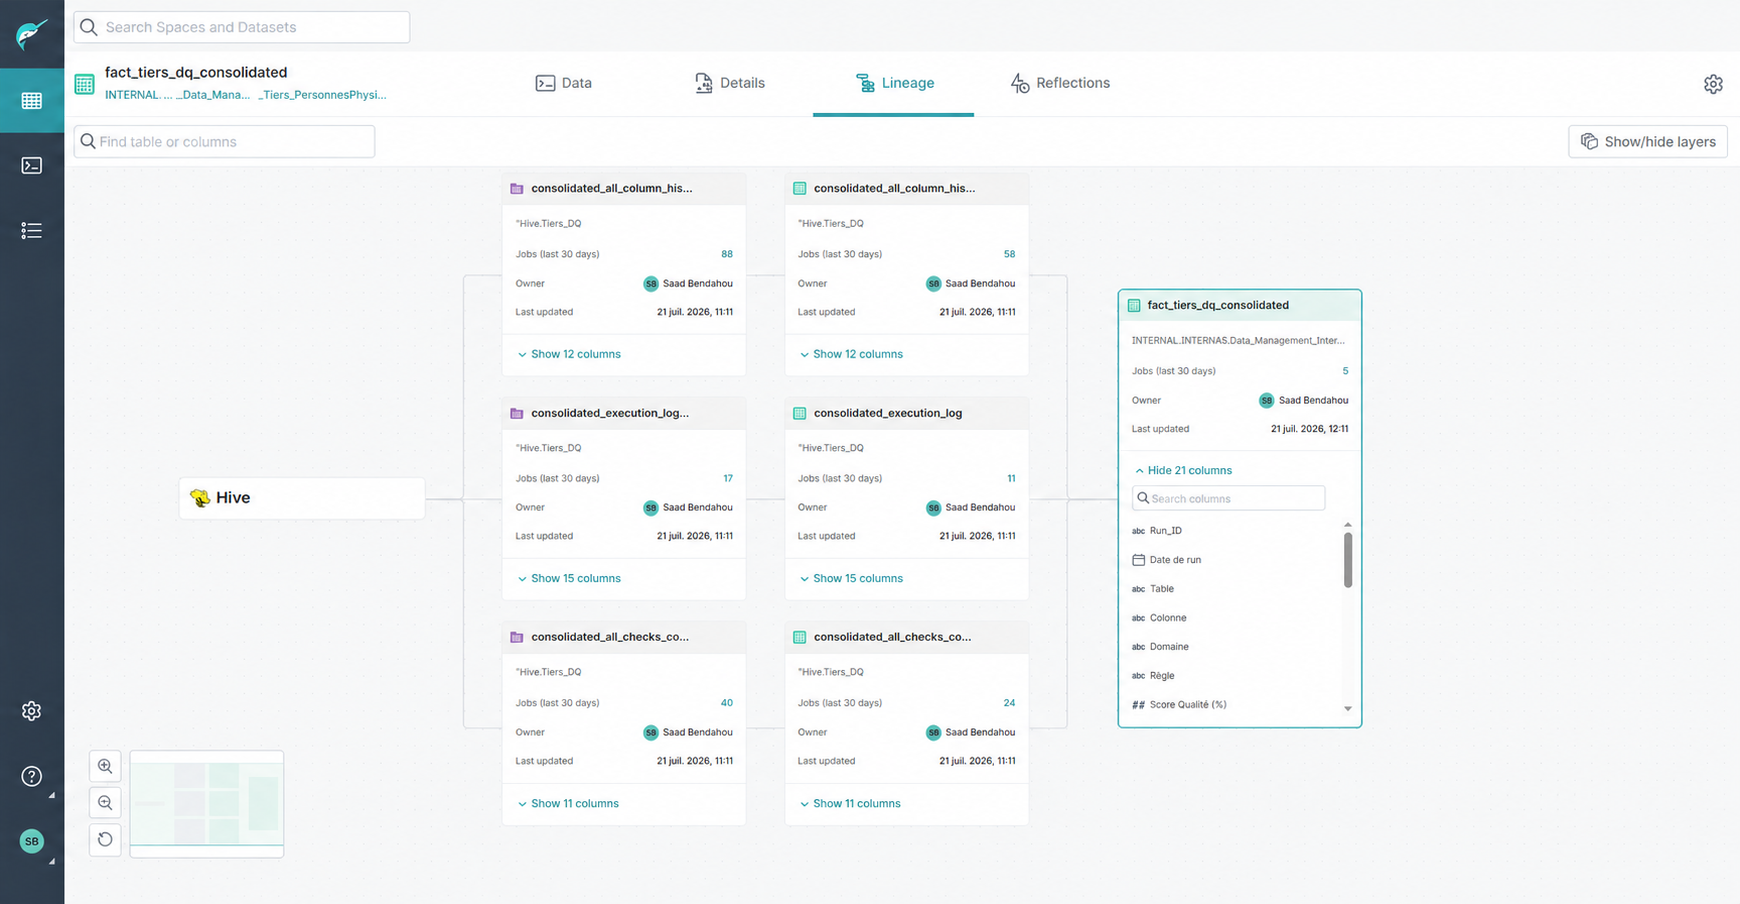
\includegraphics[width=\textwidth, keepaspectratio]{figures/lignage_dremio.png}
    \caption{Lignage des données dans Dremio montrant la création de la vue sémantique \texttt{fact\allowbreak\_tiers\allowbreak\_dq\allowbreak\_consolidated}}
    \label{fig:screenshot_dremio}
\end{figure}

Afin d'optimiser les performances de requêtage, aucune pré-agrégation lourde n'est appliquée au niveau de Dremio. L'exposition de cette grande table de faits consolidée permet de déléguer toute l'intelligence de calcul et de restitution dynamique à l'outil BI Tableau Desktop.

% =========================
\section{Réalisation du dashboard Tableau}

\subsection{Connexion Tableau à Dremio et traitement analytique}

Le dashboard Tableau est connecté à Dremio via le connecteur ODBC/JDBC natif. L'unique vue virtuelle \texttt{fact\allowbreak\_tiers\allowbreak\_dq\allowbreak\_consolidated} est importée comme source de données unique dans Tableau Desktop. 

Tous les filtres (par date d'exécution, par sous-domaine, par dimension de qualité), ainsi que toutes les agrégations (comptage de règles, calculs des moyennes de taux de conformité quotidiens ou scores moyens) sont réalisés de manière dynamique au sein des feuilles de calcul (sheets) et des tableaux de bord de Tableau en tirant directement les champs de la table de faits.


\emph{Note de confidentialité : Il est important de souligner que, pour des raisons évidentes de sécurité et de respect du secret bancaire, les noms de tables réels et certaines données sensibles présentées dans les captures d'écran suivantes ont fait l'objet d'un masquage ou d'un floutage systématique.}

\subsection{Onglet 1 — Vue d'ensemble (Dashboard Global)}

La figure \ref{fig:vuehome} présente la page d'accueil du dashboard, offrant une vision synthétique de l'état de santé du référentiel.

\begin{figure}[H]
    \centering
    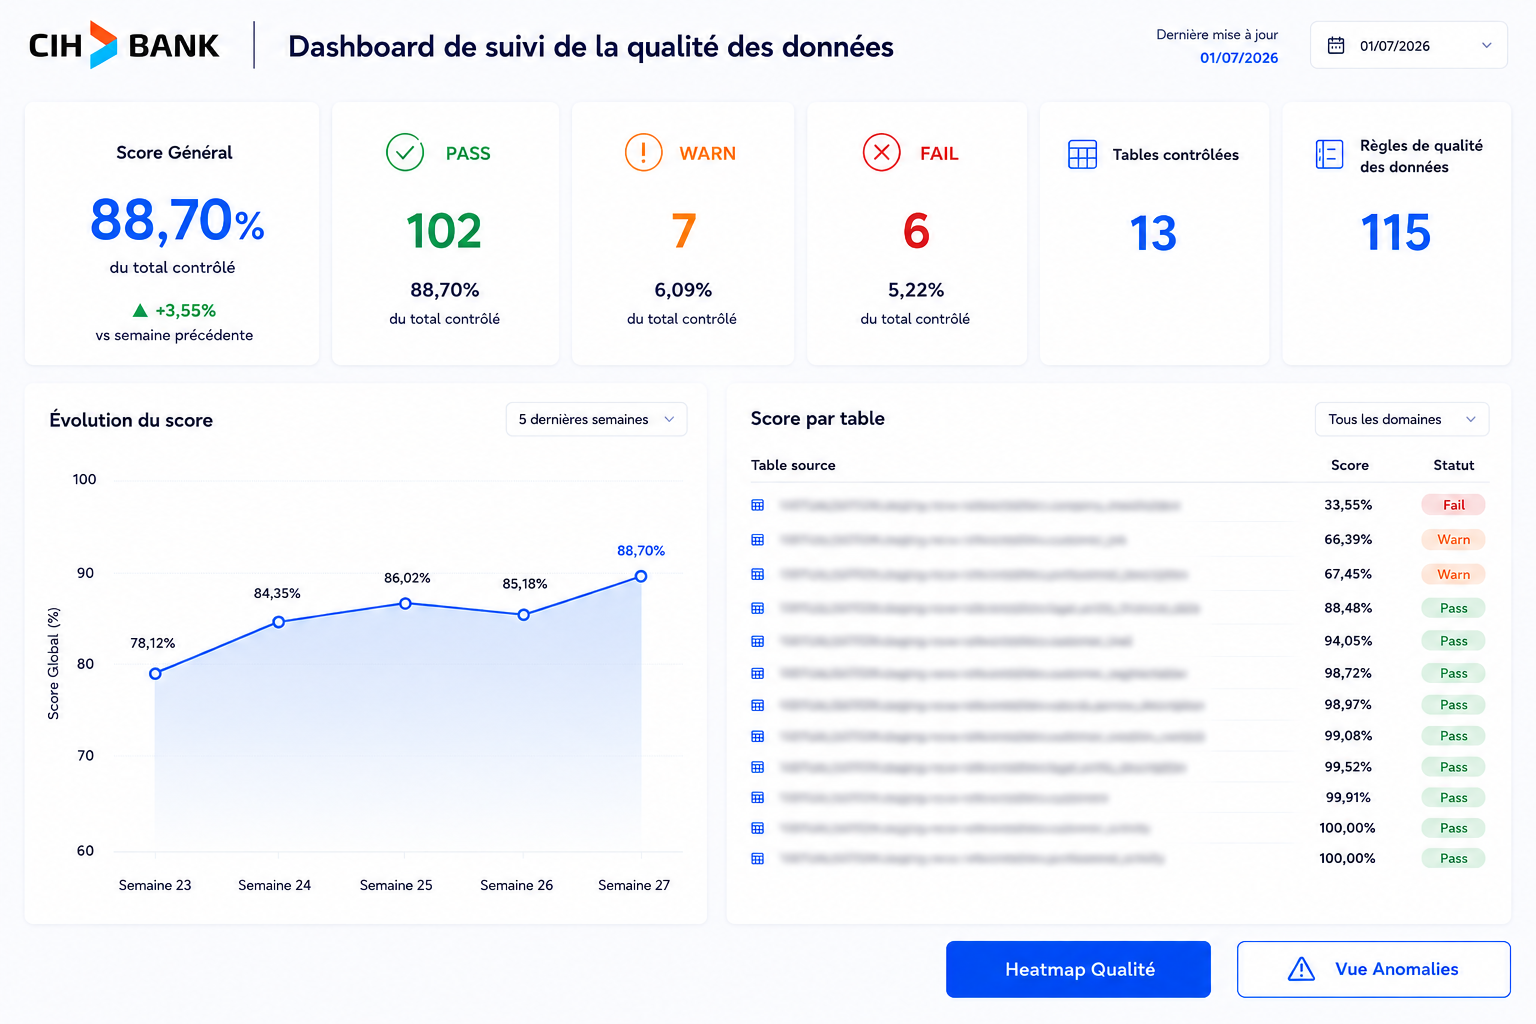
\includegraphics[width=\textwidth]{figures/vuehome.png}
    \caption{Dashboard Tableau — Vue d'ensemble de la qualité des données}
    \label{fig:vuehome}
\end{figure}

Cet onglet centralise les indicateurs de haut niveau :
\begin{itemize}
    \item Le \textbf{Score Général} de qualité (ex: 88,70\%) et sa variation par rapport à la semaine précédente.
    \item La répartition des contrôles par statut : le nombre de tests en succès (PASS), en avertissement (WARN) ou en échec (FAIL), accompagnés de leurs pourcentages respectifs.
    \item Le périmètre évalué (nombre de tables contrôlées et nombre de règles déployées).
    \item L'\textbf{Évolution du score} sur les 5 dernières semaines sous forme de graphique linéaire, permettant d'observer la tendance globale de la qualité.
    \item Un tableau de classement détaillant le \textbf{Score par table}, permettant d'identifier d'un coup d'œil les tables les plus problématiques (marquées en rouge "Fail").
\end{itemize}

\subsection{Onglet 2 — Heatmap Qualité}

La figure \ref{fig:heatmap} présente la vue matricielle détaillée.

\begin{figure}[H]
    \centering
    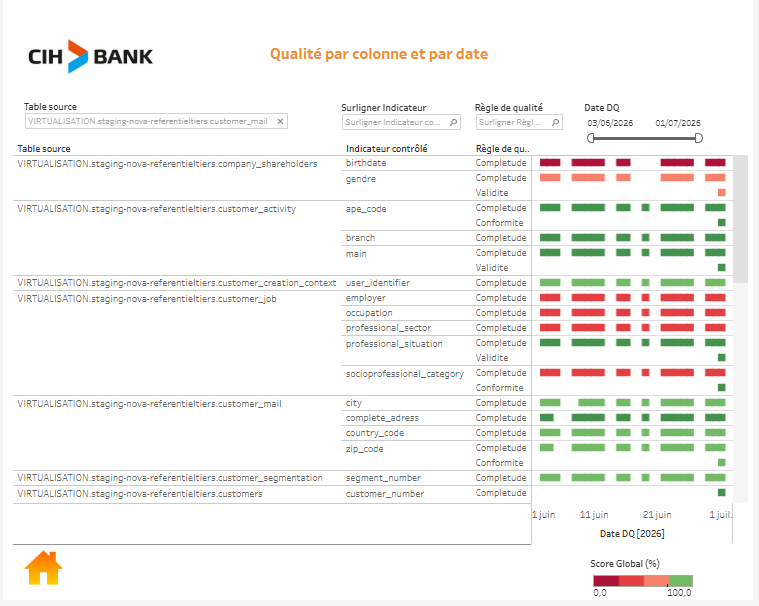
\includegraphics[width=\textwidth]{figures/HEATMAP.png}
    \caption{Dashboard Tableau — Heatmap Qualité par colonne et par date}
    \label{fig:heatmap}
\end{figure}

Cet onglet permet une analyse granulaire du niveau de qualité :
\begin{itemize}
    \item Il liste précisément chaque \textbf{Indicateur contrôlé} (ex: \texttt{birthdate}, \texttt{gender}, \texttt{city}, etc.) associé à sa \textbf{Règle de qualité} (Complétude, Validité, Conformité).
    \item Une \textbf{carte de chaleur (Heatmap) temporelle} colore les résultats par date de scan, allant du rouge (échec total) au vert (succès total). Cette visualisation est extrêmement pertinente pour repérer rapidement des dégradations soudaines (incident de pipeline) ou confirmer l'efficacité d'une campagne de remédiation des données au fil du temps.
\end{itemize}

\subsection{Onglet 3 — Top Anomalies}

La figure \ref{fig:anomaly} présente la vue orientée sur l'analyse et la remédiation.

\begin{figure}[H]
    \centering
    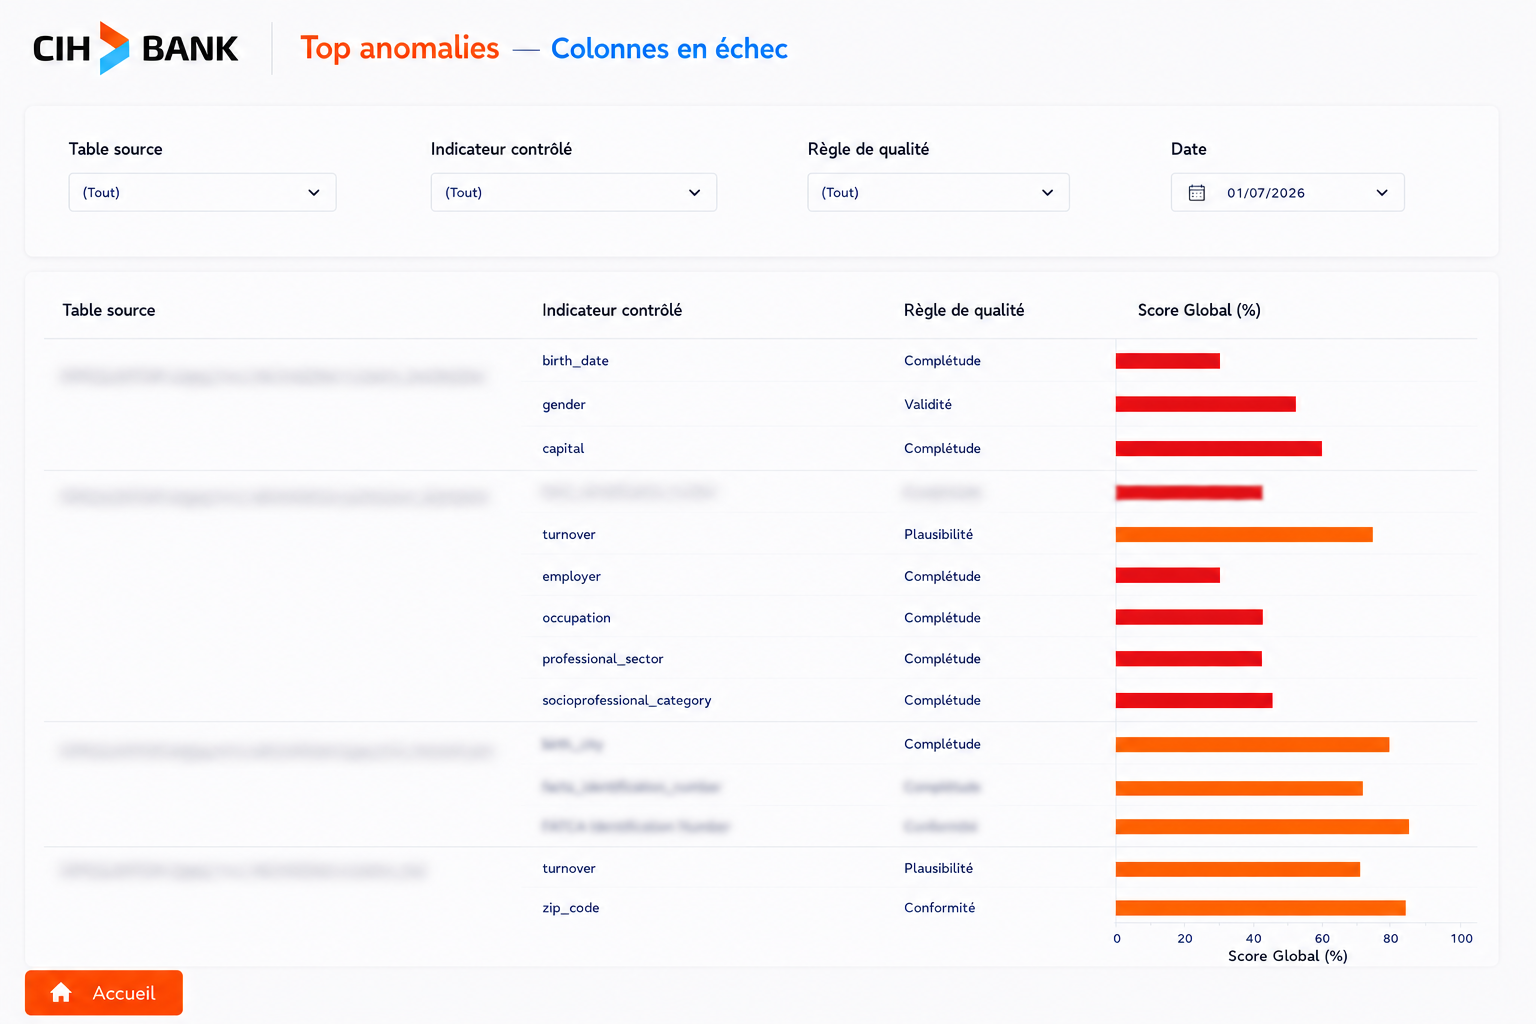
\includegraphics[width=\textwidth]{figures/anomaly.png}
    \caption{Dashboard Tableau — Top anomalies et colonnes en échec}
    \label{fig:anomaly}
\end{figure}

Ce dernier onglet est un véritable outil d'action pour les Data Stewards :
\begin{itemize}
    \item Il cible exclusivement les règles de qualité et les colonnes présentant des taux d'anomalies élevés.
    \item Un diagramme en barres horizontales présente le \textbf{Score Global (\%)} pour chaque indicateur en souffrance. Plus la barre s'approche du rouge et de 0, plus la volumétrie de données non-conformes est critique.
    \item Grâce aux filtres dynamiques situés en haut (par table, par indicateur, par règle ou par date), les utilisateurs métiers peuvent isoler instantanément les axes nécessitant des actions de correction collectives dans l'application source NOVA.
\end{itemize}

\section*{Conclusion}

Ce chapitre a présenté l'implémentation concrète des différents composants du pipeline de Data Quality Tiers : le script Soda Core avec ses fichiers de configuration YAML, les tables Hive de persistance, la tâche Airflow post-ingestion, l'exposition sémantique de Dremio et le dashboard Tableau de visualisation. L'ensemble de ces composants forme un pipeline automatisé, opérationnel chaque nuit à 22h, qui permet de mesurer, historiser et restituer la qualité des données métier du Référentiel Tiers. Le chapitre suivant présente les résultats obtenus lors des premières exécutions.


% --- Restauration du format classique pour la suite (Conclusion, Biblio) ---
\titleformat{\chapter}[display]
  {\normalfont\huge\bfseries}{\chaptertitlename\ \thechapter}{20pt}{\Huge}
\titlespacing*{\chapter}{0pt}{50pt}{40pt}

% --- Back Matter ---
\chapter*{Conclusion Générale et Perspectives}
\markboth{Conclusion Générale et Perspectives}{Conclusion Générale et Perspectives}
\addcontentsline{toc}{chapter}{Conclusion Générale et Perspectives}

\section*{Conclusion générale}
Au terme de ce projet de fin d’études, nous avons conçu, développé et industrialisé un pipeline automatisé de contrôle de la qualité des données (Data Quality) intégré à l'écosystème Big Data de CIH BANK. Ce travail répond aux problématiques rencontrées par l'institution bancaire dans la gestion de volumes de données toujours plus importants, où les traitements manuels et les opérations de remédiation curatives deviennent rapidement coûteux, chronophages et sources d’erreurs ou de non-conformité réglementaire.

L’étude préalable du contexte métier a permis d’identifier plusieurs limites des méthodes traditionnelles de gestion de la donnée, notamment l'absence de validation à la source, la difficulté d'obtenir une vision claire de l'état de santé du Data Lake, ainsi que le manque de traçabilité des anomalies liées aux informations d'identification KYC et aux catégories socio-professionnelles (CSP). Afin de répondre à ces contraintes et de se conformer aux exigences de la réglementation (loi 09-08 de la CNDP, RGPD, BCBS 239), une solution complète reposant sur des technologies modernes a été proposée et déployée.

Le pipeline développé met en œuvre une architecture robuste permettant de prendre en charge l’ensemble du cycle de fiabilisation de la donnée. Celui-ci comprend l'ingestion automatisée depuis le système source via Apache Sqoop, l'exécution distribuée de règles de qualité complexes (complétude, validité, cohérence croisée) grâce à l'intégration du framework Soda Core au sein de jobs Apache Spark, le stockage des résultats dans la zone HDFS (format ORC), ainsi que la modélisation sémantique à travers le moteur de virtualisation Dremio. L'intégration de ces résultats dans un tableau de bord interactif développé sur Tableau Software constitue également une contribution majeure, offrant aux Data Stewards un outil de supervision clair et précis.

Le projet ne s’est pas limité au développement des fonctionnalités analytiques. Une attention particulière a également été portée à l’orchestration et à l’industrialisation de la solution. La chaîne complète a été planifiée et surveillée via Apache Airflow, permettant d'automatiser le déclenchement des contrôles quotidiennement tout en s'intégrant parfaitement avec les dépendances du système d'information de la banque. Cette démarche contribue à réduire les interventions manuelles, à assurer une observabilité totale du flux de données et à garantir la fiabilité de la solution en production.

Les différents tests réalisés tout au long du projet ont permis de valider le bon fonctionnement des modules développés et leur impact positif sur l'écosystème analytique de la banque. Les objectifs fixés au début du projet ont ainsi été atteints, tout en proposant une architecture modulaire, évolutive et facilement maintenable. Au-delà des résultats obtenus, ce projet nous a permis de mettre en pratique les connaissances acquises au cours de notre formation d’ingénieur dans des domaines variés tels que le développement logiciel, l'architecture Big Data, le Data Engineering, les bases de données distribuées, la Business Intelligence ainsi que la méthodologie d'industrialisation logicielle. Cette expérience constitue une étape particulièrement enrichissante sur les plans technique et méthodologique, représentant une véritable immersion dans les exigences d’un projet industriel bancaire.

\section*{Perspectives}
Bien que les résultats obtenus soient très satisfaisants, trois perspectives d’évolution majeures peuvent être envisagées afin d’enrichir davantage la solution développée et de pousser plus loin la valorisation des données :

\paragraph{Élargissement du périmètre fonctionnel :} Actuellement centré sur le domaine des Tiers (données KYC et CSP), le pipeline a vocation à être étendu à d'autres domaines cruciaux du système d'information de CIH BANK. Il s'agirait d'intégrer les données issues du \textit{Core Banking}, notamment les écritures comptables, la comptabilité générale, ainsi que l'ensemble de la partie finance. Cette généralisation permettrait de créer une plateforme centralisée garantissant la fiabilité des données à l'échelle de toute la banque.

\paragraph{Remédiation intelligente via une approche LLM local :} Pour pallier les limites des règles purement déterministes, l'intégration de modèles de langage (LLM) exécutés localement constitue une piste prometteuse. Cette approche permettrait de remédier automatiquement à certains problèmes de qualité de données minimes ou de valeurs manquantes (par exemple, inférer contextuellement un genre à partir d'un prénom). L'exécution locale de ces modèles au sein de l'infrastructure de la banque est primordiale pour garantir la stricte confidentialité et la souveraineté des informations.

\paragraph{Intégration d'un système d'alerte multicanal intelligent :} Afin de rendre le dispositif encore plus proactif, il serait pertinent de le coupler à un système de notification multicanal (via e-mail, Microsoft Teams, etc.). Ce système serait capable d'alerter automatiquement et de manière ciblée les équipes métiers en cas de dégradation soudaine du score de qualité d'une table ou d'anomalies critiques détectées par Airflow, favorisant ainsi une réactivité immédiate sans nécessiter de surveillance manuelle continue.

Ces évolutions permettraient de faire mûrir progressivement l'infrastructure actuelle vers un système autonome et proactif, véritable centre névralgique du pilotage de la santé des données au sein de l'institution.


\chapter*{Bibliographie et Nétographie}
\addcontentsline{toc}{chapter}{Bibliographie et Nétographie}

\section*{Nétographie (Webographie)}
\begin{enumerate}
    \item \url{https://innowise.com/blog/data-analytics-in-banking/} : How data analytics is transforming the banking and financial services industry - Innowise.
    \item \url{https://scielo.org.za/scielo.php?script=sci_arttext&pid=S2304-82632024000200007} : Artificial intelligence technology to enhance data quality management practices in the banking industry in South Africa.
    \item \url{https://www.ewsolutions.com/financial-data-quality-management/} : Financial Data Quality Management: Unlocking the Power for Competitive Advantage.
    \item \url{https://www.ibm.com/new/product-blog/bcbs239-compliance} : BCBS 239 compliance: Key findings, failures and fixes with watsonx.data intelligence - IBM.
    \item \url{https://www.researchgate.net/publication/389700967_Assessing_Data_Quality_Challenges_on_International_Banking_In_Case_of_Commercial_Bank_of_Ethiopia} : (PDF) Assessing Data Quality Challenges on International Banking: In Case of Commercial Bank of Ethiopia - ResearchGate.
    \item \url{https://corp-im.com/cost-of-bad-data-decisions/} : Cost of Bad Data Decisions: Hidden Financial Damage (2026) - Corpim.
    \item \url{https://www.researchgate.net/publication/282829737_Data_quality_in_banking_regulatory_requirements_and_best_practices} : Data quality in banking: Regulatory requirements and best practices | Request PDF.
    \item \url{https://sbs-software.com/insights/artificial-intelligence-data/data-driven-transformation-banking/} : Data-driven transformation in European banking - SBS Software.
    \item \url{https://www.actian.com/blog/data-management/the-costly-consequences-of-poor-data-quality/} : The Consequences of Poor Data Quality: Uncovering the Hidden Risks - Actian Corporation.
    \item \url{https://open.metu.edu.tr/handle/11511/25576} : Data quality assessment in credit risk management by customized total data quality management approach - OpenMETU.
    \item \url{https://etd.lib.metu.edu.tr/upload/12619894/index.pdf} : data quality assessment in credit risk management by a.
    \item \url{https://www.collibra.com/blog/the-6-dimensions-of-data-quality} : The 6 Data Quality Dimensions with Examples - Collibra.
    \item \url{https://www.integrate.io/blog/data-quality-improvement-stats-from-etl/} : Data Quality Improvement Stats from ETL – 50+ Key Facts Every Data Leader Should Know in 2026 | Integrate.io.
    \item \url{https://eminence.ch/en/cost-poor-data-quality/} : The \$12.9M Drain: The Real Cost of Poor Data Quality - agence Eminence.
    \item \url{https://www.doubletrack.com/post/hidden-cost-dirty-data} : The Hidden Cost of Dirty Data: \$617B, Per Our 2026 Data Report.
    \item \url{https://veridion.com/blog-posts/banking-capital-markets-data-strategy-development/} : How to Develop a Data Strategy in Banking and Capital Markets - Veridion.
    \item \url{https://www.mdpi.com/1424-8220/25/14/4345} : Quantifying the Multidimensional Impact of Cyber Attacks in Digital Financial Services: A Systematic Literature Review - MDPI.
    \item \url{https://www.bis.org/publ/bcbs239.pdf} : Basel Committee on Banking Supervision – Principles for effective risk data aggregation and risk reporting - Bank for International Settlements.
    \item \url{https://montecarlo.ai/blog-bcbs-239-data-quality/} : BCBS 239 Data Quality Requirements: How Banks Can Ensure Compliance.
    \item \url{https://www.solidatus.com/bcbs-239/} : What is BCBS 239? A Summary of Key Principles \& Compliance - Solidatus.
    \item \url{https://www.fluxforce.ai/regulations/bcbs-bcbs-239-risk-data-aggregation/} : BCBS 239: Requirements, Scope, Penalties \& Compliance - FluxForce AI.
    \item \url{https://www.collibra.com/blog/how-to-achieve-data-quality-excellence-for-bcbs-239-risk-data-aggregation-compliance} : BCBS 239 data quality excellence for risk compliance - Collibra.
    \item \url{https://www.ey.com/en_nl/industries/banking-capital-markets/why-bcbs-239-compliance-is-essential-in-2025} : Why BCBS 239 Compliance is essential in 2025 | EY - Netherlands.
    \item \url{https://soda.io/use-cases/bcbs239-compliance} : BCBS 239 Compliance with Soda Data Quality.
    \item \url{https://iason-onigiri-prod.s3.eu-south-1.amazonaws.com/Credit_Risk_Basel_IV_Regulatory_Framework_and_New_Frontiers_8db63aced7.pdf} : Credit Risk: Basel IV Regulatory Framework and New Frontiers - AWS.
    \item \url{https://kpmg.com/xx/en/our-insights/ecb-office/ecb-ratchets-up-the-pressure-on-risk-data-aggregation.html} : ECB ratchets up the pressure on risk data aggregation - KPMG International.
    \item \url{https://www.oliverwyman.com/our-expertise/insights/2024/jul/data-management-risk-reporting-challenges-eu-banks-bcbs239.html} : Data Management And Risk Reporting Challenges For EU Banks - Oliver Wyman.
    \item \url{https://www.grantthornton.com.cy/insights/quantitative-risk-articles/ECB-Guide-on-effective-risk-data-aggregation-and-risk-reporting/} : ECB Guide on effective risk data aggregation and risk reporting - Grant Thornton Cyprus.
    \item \url{https://validio.io/blog/bcbs-239-from-regulatory-burden-to-data-quality} : BCBS 239: Turning regulatory burden into data quality excellence - Validio.
    \item \url{https://www.bairdholm.com/blog/citigroup-fined-136-million-totaling-536-million-since-2020/} : Citigroup Fined \$136 Million, Totaling \$536 Million Since 2020 | Baird Holm LLP.
    \item \url{https://www.bankingsupervision.europa.eu/press/pr/date/2026/html/ssm.pr260219~93d5b6f73e.sv.html} : ECB sanctions J.P. Morgan for misreporting capital requirements - Banking supervision.
    \item \url{https://basecapanalytics.com/the-real-cost-of-bad-data/} : Citigroup fined for bad loan data - Basecap Analytics.
    \item \url{https://www.banque-france.fr/en/press-release/ecb-sanctions-bofa-securities-europe-sa-breaching-reporting-requirements} : ECB sanctions BofA Securities Europe SA for breaching reporting requirements.
    \item \url{https://www.federalreserve.gov/newsevents/pressreleases/enforcement20240710a.htm} : Federal Reserve Board fines Citigroup \$60.6 million for violating the Board's 2020 enforcement action.
    \item \url{https://www.experian.co.uk/blogs/latest-thinking/data-quality/hidden-cost-of-untrusted-data/} : The hidden cost of untrusted data at AI scale - Experian UK.
    \item \url{https://store.ectap.ro/articole/699.pdf} : Credit Risk Assessment under Basel Accords - Theoretical and Applied Economics.
    \item \url{https://www.ibm.com/think/insights/cost-of-poor-data-quality} : The True Cost of Poor Data Quality - IBM.
    \item \url{https://www.querysurge.com/resource-center/white-papers/the-data-validation-deficit-analyzing-banking-pain-points-and-the-quest-for-effective-solutions} : White Papers - Analyzing Banking Pain Points and the Quest for Effective Solutions.
    \item \url{https://journals.co.za/doi/abs/10.7553/90-2-2392} : Artificial intelligence technology to enhance data quality management practices in the banking industry in South Africa - Sabinet African Journals.
    \item \url{https://ideas.repec.org/p/bdi/opques/qef_666_22.html} : A decision-making rule to detect insufficient data quality: an application of statistical learning techniques to the non-performing loans banking data? - IDEAS/RePEc.
    \item \url{https://barrmoses.medium.com/citigroup-fined-136m-for-bad-data-what-can-we-learn-1f15f82ea928} : Citigroup Fined \$136M for Bad Data. What Can We Learn? | by Barr Moses - Medium.
    \item \url{https://docs.soda.io/soda-core/overview-main.html} : Soda Core Official Documentation - Data Quality Management.
    \item \url{https://spark.apache.org/docs/latest/} : Apache Spark Official Documentation - Unified Engine for Large-Scale Data Analytics.
    \item \url{https://airflow.apache.org/docs/} : Apache Airflow Official Documentation - A platform to programmatically author, schedule, and monitor workflows.
    \item \url{https://docs.dremio.com/} : Dremio Documentation - The Easy and Open Data Lakehouse.
    \item \url{https://docs.python.org/3/} : Python Software Foundation - Official Documentation.
    \item \url{https://docs.cloudera.com/} : Cloudera Documentation - Enterprise Data Cloud.
\end{enumerate}


\end{document}
